\documentclass[11pt,compress,t,notes=noshow, xcolor=table]{beamer}
\usepackage[]{graphicx}\usepackage[]{color}
% maxwidth is the original width if it is less than linewidth
% otherwise use linewidth (to make sure the graphics do not exceed the margin)
\makeatletter
\def\maxwidth{ %
  \ifdim\Gin@nat@width>\linewidth
    \linewidth
  \else
    \Gin@nat@width
  \fi
}
\makeatother

\definecolor{fgcolor}{rgb}{0.345, 0.345, 0.345}
\newcommand{\hlnum}[1]{\textcolor[rgb]{0.686,0.059,0.569}{#1}}%
\newcommand{\hlstr}[1]{\textcolor[rgb]{0.192,0.494,0.8}{#1}}%
\newcommand{\hlcom}[1]{\textcolor[rgb]{0.678,0.584,0.686}{\textit{#1}}}%
\newcommand{\hlopt}[1]{\textcolor[rgb]{0,0,0}{#1}}%
\newcommand{\hlstd}[1]{\textcolor[rgb]{0.345,0.345,0.345}{#1}}%
\newcommand{\hlkwa}[1]{\textcolor[rgb]{0.161,0.373,0.58}{\textbf{#1}}}%
\newcommand{\hlkwb}[1]{\textcolor[rgb]{0.69,0.353,0.396}{#1}}%
\newcommand{\hlkwc}[1]{\textcolor[rgb]{0.333,0.667,0.333}{#1}}%
\newcommand{\hlkwd}[1]{\textcolor[rgb]{0.737,0.353,0.396}{\textbf{#1}}}%
\let\hlipl\hlkwb

\usepackage{framed}
\makeatletter
\newenvironment{kframe}{%
 \def\at@end@of@kframe{}%
 \ifinner\ifhmode%
  \def\at@end@of@kframe{\end{minipage}}%
  \begin{minipage}{\columnwidth}%
 \fi\fi%
 \def\FrameCommand##1{\hskip\@totalleftmargin \hskip-\fboxsep
 \colorbox{shadecolor}{##1}\hskip-\fboxsep
     % There is no \\@totalrightmargin, so:
     \hskip-\linewidth \hskip-\@totalleftmargin \hskip\columnwidth}%
 \MakeFramed {\advance\hsize-\width
   \@totalleftmargin\z@ \linewidth\hsize
   \@setminipage}}%
 {\par\unskip\endMakeFramed%
 \at@end@of@kframe}
\makeatother

\definecolor{shadecolor}{rgb}{.97, .97, .97}
\definecolor{messagecolor}{rgb}{0, 0, 0}
\definecolor{warningcolor}{rgb}{1, 0, 1}
\definecolor{errorcolor}{rgb}{1, 0, 0}
\newenvironment{knitrout}{}{} % an empty environment to be redefined in TeX

\usepackage{alltt}
\newcommand{\SweaveOpts}[1]{}  % do not interfere with LaTeX
\newcommand{\SweaveInput}[1]{} % because they are not real TeX commands
\newcommand{\Sexpr}[1]{}       % will only be parsed by R
\newcommand{\xmark}{\ding{55}}%


\usepackage[english]{babel}
\usepackage[utf8]{inputenc}

\usepackage{dsfont}
\usepackage{verbatim}
\usepackage{amsmath}
\usepackage{amsfonts}
\usepackage{amssymb}
\usepackage{bm}
\usepackage{csquotes}
\usepackage{multirow}
\usepackage{longtable}
\usepackage{booktabs}
\usepackage{enumerate}
\usepackage[absolute,overlay]{textpos}
\usepackage{psfrag}
\usepackage{algorithm}
\usepackage{algpseudocode}
\usepackage{eqnarray}
\usepackage{arydshln}
\usepackage{tabularx}
\usepackage{placeins}
\usepackage{tikz}
\usepackage{setspace}
\usepackage{colortbl}
\usepackage{mathtools}
\usepackage{wrapfig}
\usepackage{bm}
\usepackage{amsmath}
\usepackage{pifont}
\usepackage[round]{natbib}
\usepackage{hyperref}

\usetikzlibrary{shapes,arrows,automata,positioning,calc,chains,trees, shadows}
\tikzset{
  %Define standard arrow tip
  >=stealth',
  %Define style for boxes
  punkt/.style={
    rectangle,
    rounded corners,
    draw=black, very thick,
    text width=6.5em,
    minimum height=2em,
    text centered},
  % Define arrow style
  pil/.style={
    ->,
    thick,
    shorten <=2pt,
    shorten >=2pt,}
}

\usepackage{subfig}

% Defines macros and environments
\usepackage{../../style/lmu-lecture}


\let\code=\texttt
\let\proglang=\textsf

\setkeys{Gin}{width=0.9\textwidth}

\setbeamertemplate{frametitle}{\expandafter\uppercase\expandafter\insertframetitle}

% basic latex stuff
\newcommand{\pkg}[1]{{\fontseries{b}\selectfont #1}} % fontstyle for R packages

% Often used in exercise Rnw files, still relevant?
\newcommand{\lz}{\vspace{0.5cm}} % vertical space
\newcommand{\dlz}{\vspace{1cm}}  % double vertical space

% Unused and about to be deleted
\newcommand{\oneliner}[1] % Oneliner for important statements
{\begin{block}{}\begin{center}\begin{Large}#1\end{Large}\end{center}\end{block}}


%--------------------%
%  New environments  %
%--------------------%

 % Frame with breaks and verbatim // this is used very often
\newenvironment{vbframe}
{
\begin{frame}[containsverbatim,allowframebreaks]
}
{
\end{frame}
}

% Frame with verbatim without breaks (to avoid numbering one slided frames)
% This is not used anywhere but I can see it being useful
\newenvironment{vframe}
{
\begin{frame}[containsverbatim]
}
{
\end{frame}
}

% Itemize block
\newenvironment{blocki}[1]
{
\begin{block}{#1}\begin{itemize}
}
{
\end{itemize}\end{block}
}

%--------------%
%  Citebutton  %
%--------------%
% Example usage (from slides-cart-discussion.tex)
% \citebutton{Breiman, 1984}{https://www.taylorfrancis.com/books/mono/10.1201/9781315139470/classification-regression-trees-leo-breiman}
\newcommand{\citebutton}[2]{%
\NoCaseChange{\resizebox{!}{9pt}{\protect\beamergotobutton{\href{#2}{#1}}}}%
}

% textcolor that works in mathmode
% https://tex.stackexchange.com/a/261480
% Used e.g. in forests/slides-forests-bagging.tex
% [...] \textcolor{blue}{\tfrac{1}{M}\sum^M_{m} [...]
\makeatletter
\renewcommand*{\@textcolor}[3]{%
  \protect\leavevmode
  \begingroup
    \color#1{#2}#3%
  \endgroup
}
\makeatother





% dependencies: amsmath, amssymb, dsfont
% math spaces
\ifdefined\N
\renewcommand{\N}{\mathds{N}} % N, naturals
\else \newcommand{\N}{\mathds{N}} \fi
\newcommand{\Z}{\mathds{Z}} % Z, integers
\newcommand{\Q}{\mathds{Q}} % Q, rationals
\newcommand{\R}{\mathds{R}} % R, reals
\ifdefined\C
\renewcommand{\C}{\mathds{C}} % C, complex
\else \newcommand{\C}{\mathds{C}} \fi
\newcommand{\continuous}{\mathcal{C}} % C, space of continuous functions
\newcommand{\M}{\mathcal{M}} % machine numbers
\newcommand{\epsm}{\epsilon_m} % maximum error

% counting / finite sets
\newcommand{\setzo}{\{0, 1\}} % set 0, 1
\newcommand{\setmp}{\{-1, +1\}} % set -1, 1
\newcommand{\unitint}{[0, 1]} % unit interval

% basic math stuff
\newcommand{\xt}{\tilde x} % x tilde
\DeclareMathOperator*{\argmax}{arg\,max} % argmax
\DeclareMathOperator*{\argmin}{arg\,min} % argmin
\newcommand{\argminlim}{\mathop{\mathrm{arg\,min}}\limits} % argmax with limits
\newcommand{\argmaxlim}{\mathop{\mathrm{arg\,max}}\limits} % argmin with limits
\newcommand{\sign}{\operatorname{sign}} % sign, signum
\newcommand{\I}{\mathbb{I}} % I, indicator
\newcommand{\order}{\mathcal{O}} % O, order
\newcommand{\bigO}{\mathcal{O}} % Big-O Landau
\newcommand{\littleo}{{o}} % Little-o Landau
\newcommand{\pd}[2]{\frac{\partial{#1}}{\partial #2}} % partial derivative
\newcommand{\floorlr}[1]{\left\lfloor #1 \right\rfloor} % floor
\newcommand{\ceillr}[1]{\left\lceil #1 \right\rceil} % ceiling
\newcommand{\indep}{\perp \!\!\! \perp} % independence symbol

% sums and products
\newcommand{\sumin}{\sum\limits_{i=1}^n} % summation from i=1 to n
\newcommand{\sumim}{\sum\limits_{i=1}^m} % summation from i=1 to m
\newcommand{\sumjn}{\sum\limits_{j=1}^n} % summation from j=1 to p
\newcommand{\sumjp}{\sum\limits_{j=1}^p} % summation from j=1 to p
\newcommand{\sumik}{\sum\limits_{i=1}^k} % summation from i=1 to k
\newcommand{\sumkg}{\sum\limits_{k=1}^g} % summation from k=1 to g
\newcommand{\sumjg}{\sum\limits_{j=1}^g} % summation from j=1 to g
\newcommand{\meanin}{\frac{1}{n} \sum\limits_{i=1}^n} % mean from i=1 to n
\newcommand{\meanim}{\frac{1}{m} \sum\limits_{i=1}^m} % mean from i=1 to n
\newcommand{\meankg}{\frac{1}{g} \sum\limits_{k=1}^g} % mean from k=1 to g
\newcommand{\prodin}{\prod\limits_{i=1}^n} % product from i=1 to n
\newcommand{\prodkg}{\prod\limits_{k=1}^g} % product from k=1 to g
\newcommand{\prodjp}{\prod\limits_{j=1}^p} % product from j=1 to p

% linear algebra
\newcommand{\one}{\bm{1}} % 1, unitvector
\newcommand{\zero}{\mathbf{0}} % 0-vector
\newcommand{\id}{\bm{I}} % I, identity
\newcommand{\diag}{\operatorname{diag}} % diag, diagonal
\newcommand{\trace}{\operatorname{tr}} % tr, trace
\newcommand{\spn}{\operatorname{span}} % span
\newcommand{\scp}[2]{\left\langle #1, #2 \right\rangle} % <.,.>, scalarproduct
\newcommand{\mat}[1]{\begin{pmatrix} #1 \end{pmatrix}} % short pmatrix command
\newcommand{\Amat}{\mathbf{A}} % matrix A
\newcommand{\Deltab}{\mathbf{\Delta}} % error term for vectors

% basic probability + stats
\renewcommand{\P}{\mathds{P}} % P, probability
\newcommand{\E}{\mathds{E}} % E, expectation
\newcommand{\var}{\mathsf{Var}} % Var, variance
\newcommand{\cov}{\mathsf{Cov}} % Cov, covariance
\newcommand{\corr}{\mathsf{Corr}} % Corr, correlation
\newcommand{\normal}{\mathcal{N}} % N of the normal distribution
\newcommand{\iid}{\overset{i.i.d}{\sim}} % dist with i.i.d superscript
\newcommand{\distas}[1]{\overset{#1}{\sim}} % ... is distributed as ...

% machine learning
\newcommand{\Xspace}{\mathcal{X}} % X, input space
\newcommand{\Yspace}{\mathcal{Y}} % Y, output space
\newcommand{\Zspace}{\mathcal{Z}} % Z, space of sampled datapoints
\newcommand{\nset}{\{1, \ldots, n\}} % set from 1 to n
\newcommand{\pset}{\{1, \ldots, p\}} % set from 1 to p
\newcommand{\gset}{\{1, \ldots, g\}} % set from 1 to g
\newcommand{\Pxy}{\mathbb{P}_{xy}} % P_xy
\newcommand{\Exy}{\mathbb{E}_{xy}} % E_xy: Expectation over random variables xy
\newcommand{\xv}{\mathbf{x}} % vector x (bold)
\newcommand{\xtil}{\tilde{\mathbf{x}}} % vector x-tilde (bold)
\newcommand{\yv}{\mathbf{y}} % vector y (bold)
\newcommand{\xy}{(\xv, y)} % observation (x, y)
\newcommand{\xvec}{\left(x_1, \ldots, x_p\right)^\top} % (x1, ..., xp)
\newcommand{\Xmat}{\mathbf{X}} % Design matrix
\newcommand{\allDatasets}{\mathds{D}} % The set of all datasets
\newcommand{\allDatasetsn}{\mathds{D}_n}  % The set of all datasets of size n
\newcommand{\D}{\mathcal{D}} % D, data
\newcommand{\Dn}{\D_n} % D_n, data of size n
\newcommand{\Dtrain}{\mathcal{D}_{\text{train}}} % D_train, training set
\newcommand{\Dtest}{\mathcal{D}_{\text{test}}} % D_test, test set
\newcommand{\xyi}[1][i]{\left(\xv^{(#1)}, y^{(#1)}\right)} % (x^i, y^i), i-th observation
\newcommand{\Dset}{\left( \xyi[1], \ldots, \xyi[n]\right)} % {(x1,y1)), ..., (xn,yn)}, data
\newcommand{\defAllDatasetsn}{(\Xspace \times \Yspace)^n} % Def. of the set of all datasets of size n
\newcommand{\defAllDatasets}{\bigcup_{n \in \N}(\Xspace \times \Yspace)^n} % Def. of the set of all datasets
\newcommand{\xdat}{\left\{ \xv^{(1)}, \ldots, \xv^{(n)}\right\}} % {x1, ..., xn}, input data
\newcommand{\ydat}{\left\{ \yv^{(1)}, \ldots, \yv^{(n)}\right\}} % {y1, ..., yn}, input data
\newcommand{\yvec}{\left(y^{(1)}, \hdots, y^{(n)}\right)^\top} % (y1, ..., yn), vector of outcomes
\newcommand{\greekxi}{\xi} % Greek letter xi
\renewcommand{\xi}[1][i]{\xv^{(#1)}} % x^i, i-th observed value of x
\newcommand{\yi}[1][i]{y^{(#1)}} % y^i, i-th observed value of y
\newcommand{\xivec}{\left(x^{(i)}_1, \ldots, x^{(i)}_p\right)^\top} % (x1^i, ..., xp^i), i-th observation vector
\newcommand{\xj}{\xv_j} % x_j, j-th feature
\newcommand{\xjvec}{\left(x^{(1)}_j, \ldots, x^{(n)}_j\right)^\top} % (x^1_j, ..., x^n_j), j-th feature vector
\newcommand{\phiv}{\mathbf{\phi}} % Basis transformation function phi
\newcommand{\phixi}{\mathbf{\phi}^{(i)}} % Basis transformation of xi: phi^i := phi(xi)

%%%%%% ml - models general
\newcommand{\lamv}{\bm{\lambda}} % lambda vector, hyperconfiguration vector
\newcommand{\Lam}{\bm{\Lambda}}	 % Lambda, space of all hpos
% Inducer / Inducing algorithm
\newcommand{\preimageInducer}{\left(\defAllDatasets\right)\times\Lam} % Set of all datasets times the hyperparameter space
\newcommand{\preimageInducerShort}{\allDatasets\times\Lam} % Set of all datasets times the hyperparameter space
% Inducer / Inducing algorithm
\newcommand{\ind}{\mathcal{I}} % Inducer, inducing algorithm, learning algorithm

% continuous prediction function f
\newcommand{\ftrue}{f_{\text{true}}}  % True underlying function (if a statistical model is assumed)
\newcommand{\ftruex}{\ftrue(\xv)} % True underlying function (if a statistical model is assumed)
\newcommand{\fx}{f(\xv)} % f(x), continuous prediction function
\newcommand{\fdomains}{f: \Xspace \rightarrow \R^g} % f with domain and co-domain
\newcommand{\Hspace}{\mathcal{H}} % hypothesis space where f is from
\newcommand{\fbayes}{f^{\ast}} % Bayes-optimal model
\newcommand{\fxbayes}{f^{\ast}(\xv)} % Bayes-optimal model
\newcommand{\fkx}[1][k]{f_{#1}(\xv)} % f_j(x), discriminant component function
\newcommand{\fh}{\hat{f}} % f hat, estimated prediction function
\newcommand{\fxh}{\fh(\xv)} % fhat(x)
\newcommand{\fxt}{f(\xv ~|~ \thetav)} % f(x | theta)
\newcommand{\fxi}{f\left(\xv^{(i)}\right)} % f(x^(i))
\newcommand{\fxih}{\hat{f}\left(\xv^{(i)}\right)} % f(x^(i))
\newcommand{\fxit}{f\left(\xv^{(i)} ~|~ \thetav\right)} % f(x^(i) | theta)
\newcommand{\fhD}{\fh_{\D}} % fhat_D, estimate of f based on D
\newcommand{\fhDtrain}{\fh_{\Dtrain}} % fhat_Dtrain, estimate of f based on D
\newcommand{\fhDnlam}{\fh_{\Dn, \lamv}} %model learned on Dn with hp lambda
\newcommand{\fhDlam}{\fh_{\D, \lamv}} %model learned on D with hp lambda
\newcommand{\fhDnlams}{\fh_{\Dn, \lamv^\ast}} %model learned on Dn with optimal hp lambda
\newcommand{\fhDlams}{\fh_{\D, \lamv^\ast}} %model learned on D with optimal hp lambda

% discrete prediction function h
\newcommand{\hx}{h(\xv)} % h(x), discrete prediction function
\newcommand{\hh}{\hat{h}} % h hat
\newcommand{\hxh}{\hat{h}(\xv)} % hhat(x)
\newcommand{\hxt}{h(\xv | \thetav)} % h(x | theta)
\newcommand{\hxi}{h\left(\xi\right)} % h(x^(i))
\newcommand{\hxit}{h\left(\xi ~|~ \thetav\right)} % h(x^(i) | theta)
\newcommand{\hbayes}{h^{\ast}} % Bayes-optimal classification model
\newcommand{\hxbayes}{h^{\ast}(\xv)} % Bayes-optimal classification model

% yhat
\newcommand{\yh}{\hat{y}} % yhat for prediction of target
\newcommand{\yih}{\hat{y}^{(i)}} % yhat^(i) for prediction of ith targiet
\newcommand{\resi}{\yi- \yih}

% theta
\newcommand{\thetah}{\hat{\theta}} % theta hat
\newcommand{\thetav}{\bm{\theta}} % theta vector
\newcommand{\thetavh}{\bm{\hat\theta}} % theta vector hat
\newcommand{\thetat}[1][t]{\thetav^{[#1]}} % theta^[t] in optimization
\newcommand{\thetatn}[1][t]{\thetav^{[#1 +1]}} % theta^[t+1] in optimization
\newcommand{\thetahDnlam}{\thetavh_{\Dn, \lamv}} %theta learned on Dn with hp lambda
\newcommand{\thetahDlam}{\thetavh_{\D, \lamv}} %theta learned on D with hp lambda
\newcommand{\mint}{\min_{\thetav \in \Theta}} % min problem theta
\newcommand{\argmint}{\argmin_{\thetav \in \Theta}} % argmin theta

% densities + probabilities
% pdf of x
\newcommand{\pdf}{p} % p
\newcommand{\pdfx}{p(\xv)} % p(x)
\newcommand{\pixt}{\pi(\xv~|~ \thetav)} % pi(x|theta), pdf of x given theta
\newcommand{\pixit}[1][i]{\pi\left(\xi[#1] ~|~ \thetav\right)} % pi(x^i|theta), pdf of x given theta
\newcommand{\pixii}[1][i]{\pi\left(\xi[#1]\right)} % pi(x^i), pdf of i-th x

% pdf of (x, y)
\newcommand{\pdfxy}{p(\xv,y)} % p(x, y)
\newcommand{\pdfxyt}{p(\xv, y ~|~ \thetav)} % p(x, y | theta)
\newcommand{\pdfxyit}{p\left(\xi, \yi ~|~ \thetav\right)} % p(x^(i), y^(i) | theta)

% pdf of x given y
\newcommand{\pdfxyk}[1][k]{p(\xv | y= #1)} % p(x | y = k)
\newcommand{\lpdfxyk}[1][k]{\log p(\xv | y= #1)} % log p(x | y = k)
\newcommand{\pdfxiyk}[1][k]{p\left(\xi | y= #1 \right)} % p(x^i | y = k)

% prior probabilities
\newcommand{\pik}[1][k]{\pi_{#1}} % pi_k, prior
\newcommand{\lpik}[1][k]{\log \pi_{#1}} % log pi_k, log of the prior
\newcommand{\pit}{\pi(\thetav)} % Prior probability of parameter theta

% posterior probabilities
\newcommand{\post}{\P(y = 1 ~|~ \xv)} % P(y = 1 | x), post. prob for y=1
\newcommand{\postk}[1][k]{\P(y = #1 ~|~ \xv)} % P(y = k | y), post. prob for y=k
\newcommand{\pidomains}{\pi: \Xspace \rightarrow \unitint} % pi with domain and co-domain
\newcommand{\pibayes}{\pi^{\ast}} % Bayes-optimal classification model
\newcommand{\pixbayes}{\pi^{\ast}(\xv)} % Bayes-optimal classification model
\newcommand{\pix}{\pi(\xv)} % pi(x), P(y = 1 | x)
\newcommand{\piv}{\bm{\pi}} % pi, bold, as vector
\newcommand{\pikx}[1][k]{\pi_{#1}(\xv)} % pi_k(x), P(y = k | x)
\newcommand{\pikxt}[1][k]{\pi_{#1}(\xv ~|~ \thetav)} % pi_k(x | theta), P(y = k | x, theta)
\newcommand{\pixh}{\hat \pi(\xv)} % pi(x) hat, P(y = 1 | x) hat
\newcommand{\pikxh}[1][k]{\hat \pi_{#1}(\xv)} % pi_k(x) hat, P(y = k | x) hat
\newcommand{\pixih}{\hat \pi(\xi)} % pi(x^(i)) with hat
\newcommand{\pikxih}[1][k]{\hat \pi_{#1}(\xi)} % pi_k(x^(i)) with hat
\newcommand{\pdfygxt}{p(y ~|~\xv, \thetav)} % p(y | x, theta)
\newcommand{\pdfyigxit}{p\left(\yi ~|~\xi, \thetav\right)} % p(y^i |x^i, theta)
\newcommand{\lpdfygxt}{\log \pdfygxt } % log p(y | x, theta)
\newcommand{\lpdfyigxit}{\log \pdfyigxit} % log p(y^i |x^i, theta)

% probababilistic
\newcommand{\bayesrulek}[1][k]{\frac{\P(\xv | y= #1) \P(y= #1)}{\P(\xv)}} % Bayes rule
\newcommand{\muk}{\bm{\mu_k}} % mean vector of class-k Gaussian (discr analysis)

% residual and margin
\newcommand{\eps}{\epsilon} % residual, stochastic
\newcommand{\epsv}{\bm{\epsilon}} % residual, stochastic, as vector
\newcommand{\epsi}{\epsilon^{(i)}} % epsilon^i, residual, stochastic
\newcommand{\epsh}{\hat{\epsilon}} % residual, estimated
\newcommand{\epsvh}{\hat{\epsv}} % residual, estimated, vector
\newcommand{\yf}{y \fx} % y f(x), margin
\newcommand{\yfi}{\yi \fxi} % y^i f(x^i), margin
\newcommand{\Sigmah}{\hat \Sigma} % estimated covariance matrix
\newcommand{\Sigmahj}{\hat \Sigma_j} % estimated covariance matrix for the j-th class

% ml - loss, risk, likelihood
\newcommand{\Lyf}{L\left(y, f\right)} % L(y, f), loss function
\newcommand{\Lypi}{L\left(y, \pi\right)} % L(y, pi), loss function
\newcommand{\Lxy}{L\left(y, \fx\right)} % L(y, f(x)), loss function
\newcommand{\Lxyi}{L\left(\yi, \fxi\right)} % loss of observation
\newcommand{\Lxyt}{L\left(y, \fxt\right)} % loss with f parameterized
\newcommand{\Lxyit}{L\left(\yi, \fxit\right)} % loss of observation with f parameterized
\newcommand{\Lxym}{L\left(\yi, f\left(\bm{\tilde{x}}^{(i)} ~|~ \thetav\right)\right)} % loss of observation with f parameterized
\newcommand{\Lpixy}{L\left(y, \pix\right)} % loss in classification
\newcommand{\Lpiv}{L\left(y, \piv\right)} % loss in classification
\newcommand{\Lpixyi}{L\left(\yi, \pixii\right)} % loss of observation in classification
\newcommand{\Lpixyt}{L\left(y, \pixt\right)} % loss with pi parameterized
\newcommand{\Lpixyit}{L\left(\yi, \pixit\right)} % loss of observation with pi parameterized
\newcommand{\Lhxy}{L\left(y, \hx\right)} % L(y, h(x)), loss function on discrete classes
\newcommand{\Lr}{L\left(r\right)} % L(r), loss defined on residual (reg) / margin (classif)
\newcommand{\lone}{|y - \fx|} % L1 loss
\newcommand{\ltwo}{\left(y - \fx\right)^2} % L2 loss
\newcommand{\lbernoullimp}{\ln(1 + \exp(-y \cdot \fx))} % Bernoulli loss for -1, +1 encoding
\newcommand{\lbernoullizo}{- y \cdot \fx + \log(1 + \exp(\fx))} % Bernoulli loss for 0, 1 encoding
\newcommand{\lcrossent}{- y \log \left(\pix\right) - (1 - y) \log \left(1 - \pix\right)} % cross-entropy loss
\newcommand{\lbrier}{\left(\pix - y \right)^2} % Brier score
\newcommand{\risk}{\mathcal{R}} % R, risk
\newcommand{\riskbayes}{\mathcal{R}^\ast}
\newcommand{\riskf}{\risk(f)} % R(f), risk
\newcommand{\riskdef}{\E_{y|\xv}\left(\Lxy \right)} % risk def (expected loss)
\newcommand{\riskt}{\mathcal{R}(\thetav)} % R(theta), risk
\newcommand{\riske}{\mathcal{R}_{\text{emp}}} % R_emp, empirical risk w/o factor 1 / n
\newcommand{\riskeb}{\bar{\mathcal{R}}_{\text{emp}}} % R_emp, empirical risk w/ factor 1 / n
\newcommand{\riskef}{\riske(f)} % R_emp(f)
\newcommand{\risket}{\mathcal{R}_{\text{emp}}(\thetav)} % R_emp(theta)
\newcommand{\riskr}{\mathcal{R}_{\text{reg}}} % R_reg, regularized risk
\newcommand{\riskrt}{\mathcal{R}_{\text{reg}}(\thetav)} % R_reg(theta)
\newcommand{\riskrf}{\riskr(f)} % R_reg(f)
\newcommand{\riskrth}{\hat{\mathcal{R}}_{\text{reg}}(\thetav)} % hat R_reg(theta)
\newcommand{\risketh}{\hat{\mathcal{R}}_{\text{emp}}(\thetav)} % hat R_emp(theta)
\newcommand{\LL}{\mathcal{L}} % L, likelihood
\newcommand{\LLt}{\mathcal{L}(\thetav)} % L(theta), likelihood
\newcommand{\LLtx}{\mathcal{L}(\thetav | \xv)} % L(theta|x), likelihood
\newcommand{\logl}{\ell} % l, log-likelihood
\newcommand{\loglt}{\logl(\thetav)} % l(theta), log-likelihood
\newcommand{\logltx}{\logl(\thetav | \xv)} % l(theta|x), log-likelihood
\newcommand{\errtrain}{\text{err}_{\text{train}}} % training error
\newcommand{\errtest}{\text{err}_{\text{test}}} % test error
\newcommand{\errexp}{\overline{\text{err}_{\text{test}}}} % avg training error

% lm
\newcommand{\thx}{\thetav^\top \xv} % linear model
\newcommand{\olsest}{(\Xmat^\top \Xmat)^{-1} \Xmat^\top \yv} % OLS estimator in LM


\newcommand{\sens}{\mathbf{A}} % vector x (bold)
\newcommand{\ba}{\mathbf{a}}
\newcommand{\batilde}{\tilde{\mathbf{a}}}
\newcommand{\Px}{\mathbb{P}_{x}} % P_x
\newcommand{\Pxj}{\mathbb{P}_{x_j}} % P_{x_j}
\newcommand{\indep}{\perp \!\!\! \perp} % independence symbol

\usepackage{multicol}

\newcommand{\titlefigure}{figure/fairness_logo.PNG}
\newcommand{\learninggoals}{
  \item Know why fairness aspects are relevant for Machine Learning
  \item Get familar with prevalent fairness criteria
  \item Know their disadvantages and their relationship
}

\title{Advanced Machine Learning}
\date{}

\begin{document}

\lecturechapter{Fairness in Machine Learning}
\lecture{Advanced Machine Learning}



\sloppy

\begin{vbframe}{Ethical aspects in Machine Learning}
%
  \begin{itemize}
%  	
    \item Machine learning methods are more and more applied in real-life application, especially for automated decision making:
%
    \begin{itemize}
%    	
		\item Credit scoring and insurance applications --- Should the credit/insurance be granted to a certain person or not?
%		
		\item Rating job applications --- Machine learning models can help filter applications much more effectively than simple keyword-based approaches.
%		
		\item Law ---  In legal systems around the world, algorithmic tools such as risk assessment instruments (RAI), are being used to supplement or replace the human judgment of judges, civil servants and police officers in many contexts. 
%		
		\item Economics --- Automated trading systems buy and sell orders and automatically transmit the orders to market centers or exchanges. 
%		
		\item $\ldots$
%    	
    \end{itemize}
%
  \end{itemize}
%
\end{vbframe}

\begin{vbframe}{Ethical aspects in Machine Learning}
%	
	\begin{itemize}
%		
		\item These are critical applications involving humans, which raises various ethical issues in different dimensions:
%		
		\begin{itemize}
			%    	
			\item Accountability --- Can we make sure that the system is functioning as intended?
%			
			\item Explainability/Transparency: Is it evident or explainable why one specific decision was made rather than another?
%			
			\item Fairness --- Does the system disadvantage specific individuals or groups?
%			
			\item Privacy --- Is the information (data) on the basis of which the system was developed secure against external access?
%			
			\item Security --- Is it possible to attack the system, e.g. by ``poisoning'' the data so that undesirable effects occur?
			%    	
		\end{itemize}
%	
	\item It should be noted that all of these aspects are intertwined in some way and becoming increasingly important from a legal perspective, e.g.\ due to the \emph{European ethics guidelines for trustworthy AI}.
%
	\end{itemize}
%
\end{vbframe}

\frame{
\frametitle{Fairness in Machine Learning: Why bother?}
%
\small
%
\begin{itemize}
%
 	\item  In the recent past, there have been a number of automated decision making tools that have attracted attention for discriminatory behavior:
 	
 	
 	\begin{multicols}{2}
 		\small
	\begin{itemize}
%  
%		
%	\begin{minipage}{0.5\textwidth}
		\footnotesize
		\item Correctional Offender Management Profiling for Alternative Sanctions (COMPAS) is a tool used by U.S.\ courts to assess the likelihood of a defendant becoming a recidivist. But there is strong evidence that it is discriminating black defendants.
%	\end{minipage}
%
%	\begin{minipage}{0.3\textwidth}
		\begin{center}			
			\includegraphics[width=0.35\textwidth]{figure/compas_article}
		\end{center}
%	\end{minipage}
%  
%	\begin{minipage}{0.5\textwidth}
%	\small
	\item Amazon created a tool to trawl the web and spot potential candidates, rating them from one to five stars. But the algorithm learned to systematically downgrade women's CV's for technical jobs such as software developer. 
%	\end{minipage}
	%
%	\begin{minipage}{0.3\textwidth}
		\begin{center}			
			
\includegraphics[width=0.4\textwidth]{figure/amazon_article}
		\end{center}
%	\end{minipage}
%
    \end{itemize}
%
\end{multicols}
\end{itemize}
%
}
 

\begin{vbframe}{Research on Fairness}
%
	\small
	\begin{itemize}
		%	
		\item The question of what fairness actually is goes back thousands of years to antiquity. Even back then, philosophers such as Aristotle asked themselves this question.
		%
	\end{itemize}
	%
	\begin{minipage}{0.5\textwidth}
	%	
		\begin{itemize}
			%	
			\item The academic research on fairness started with the pioneering works in educational testing (Clearly, 1968) and economics (Becker 1957, Phelps 1972, Arrow 1973).
			%	
			\item In computer science, the research essentially started in the early 2000s and has recently attracted a lot of interest, which is of course due to the increasing use of machine learning models for automated decision making systems.
			%	
		\end{itemize}
	%	
	\end{minipage}
	\begin{minipage}{0.45\textwidth}
	%	
		\begin{figure}
			\centering
			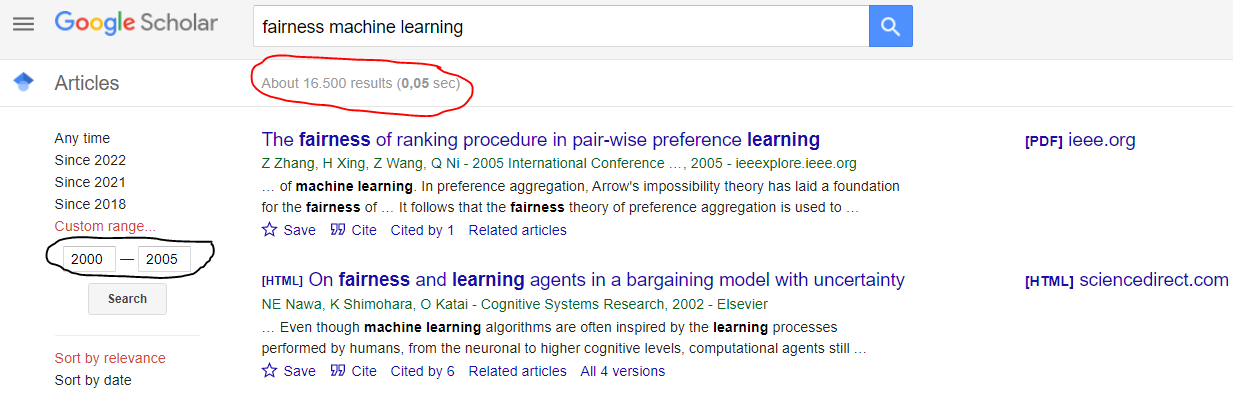
\includegraphics[width=0.99\linewidth]{figure/fairness_research_1}
			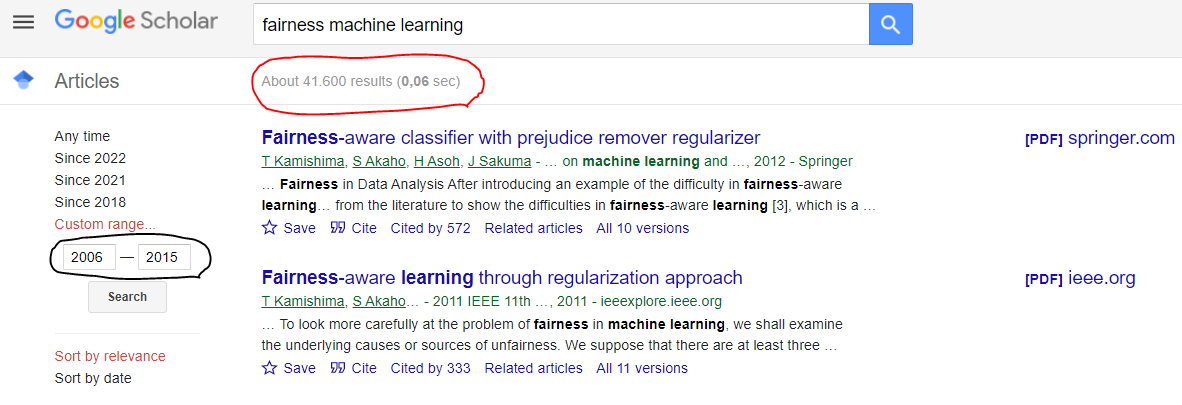
\includegraphics[width=0.99\linewidth]{figure/fairness_research_2}
			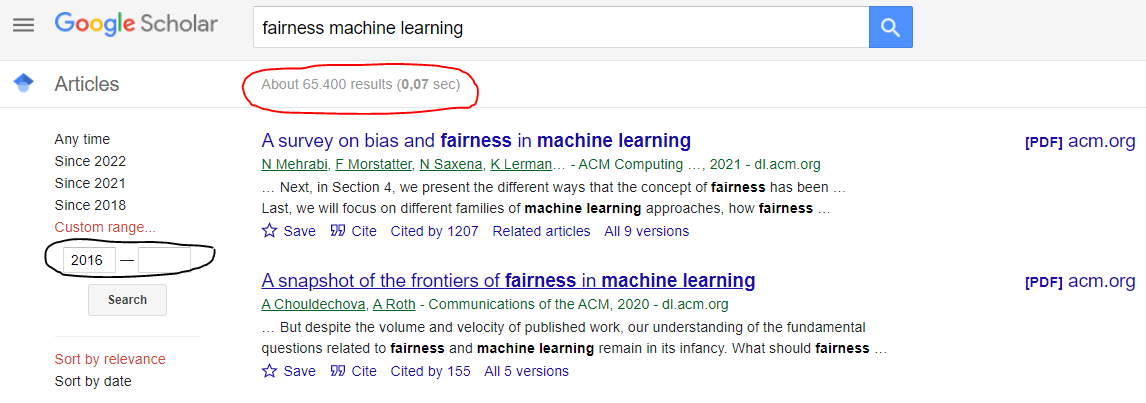
\includegraphics[width=0.99\linewidth]{figure/fairness_research_3}
		\end{figure}
	%	
	\end{minipage}
%
\end{vbframe} 

\begin{vbframe}{Fairness in Machine Learning: Rough Overview}
%
  \begin{itemize}
%    
    \item The goal of fairness in Machine Learning is, roughly speaking, to identify and mitigate or even prevent biases of any kind in the decision making based on ML methods along all aspects of the pipeline.
%    
	\item There are essentially two sources of bias, namely the available data and the ML model itself:
%	
	\begin{itemize}
%		
		\item Data can be imbalanced or impoverished, e.g.\ more data on white recidivism outcomes than for blacks. The data can be biased, e.g.\ collected by a racist or chauvinistic hiring manager. Finally, inconsistencies in the data such as wrong labels or simply noise can lead to bias as well.
%		
		\item The prediction of the ML method can be imbalanced w.r.t.\ to the error. Moreover, the ML method might mimic the biases in the data and even compound injustices.
%
	\end{itemize}
%
  \end{itemize}
%
\end{vbframe}

\begin{vbframe}{Fairness-aware binary classification}
%	
\begin{itemize}
%	
\small
\item  We will consider only the binary classification/prediction setting in this course, due to the following reasons:
%\\
	\begin{enumerate}
		\small
%		
		\item The majority of fairness-critical applications in real life are in fact binary classification/prediction tasks, e.g.\ credit application (granting vs.\ not granting a loan), job application (hire applicant or not), trading systems (buy or sell an order), $\ldots$
%		
		\item Quantifying fairness based on a binary outcome variable is mathematically more convenient, while the multi-class
		variant would introduce additional terms in the fairness quantities. Moreover, multiclass problems can (and are) often addressed by reducing them into multiple binary classification tasks, e.g.\ one-vs-rest, one-vs-one or error-correcting-codes approaches.
%
		\item The principles for fairness-aware regression tasks are often just modifications of the ones for binary classification.
%
	\end{enumerate}
%    
\end{itemize} 
%
\end{vbframe}


\begin{vbframe}{Fairness-aware binary classification: Formal setting}
%	
\scriptsize{
%
We are provided with a data set 
%
$\D = \Dset \in \defAllDatasetsn,$
%
where 
%
\begin{itemize}
%	
	\item $\Xspace$ is the input/feature/attribute space with $p = \text{dim}(\Xspace),$ 
%	
	\item $\Yspace$ the output / target / label space (for now $\Yspace = \{-1,1\}$),
%	
	\item the tuple \(\xyi\) $\in \Xspace\times \Yspace$ is the \(i\)-th observation,
%	
	\item $\xj = \xjvec$ the j-th feature vector.
%	
\end{itemize}
%
So we have observed $n$ objects, described by $p$ features.
%
\begin{itemize}
%	
	\item We assume the observed data $\D$ to be generated by a process that can
	be characterized by some probability distribution $\Pxy,$ defined on 
	$\Xspace \times \Yspace.$
%	
	\item In particular, $\Dset$ is i.i.d.\ with $\xyi\sim\Pxy $.
%	
	\item We denote the random variables (vectors) following this 
	distribution by lowercase $\xv$ and $y$.
%	
\end{itemize}
%
\begin{minipage}{0.5\textwidth}
%	
	The ultimate goal for a machine learning model $f$ is then loosely speaking `` to predict $y$ from $\xv$'', which leads to a decision $f(\xv) = \yh \in \{-1,1\}.$ Note that $\yh$ is a random variable (can be constant), as it is essentially a function of the random input $\xv.$
%	
\end{minipage}
\begin{minipage}{0.45\textwidth}
	\begin{center}
		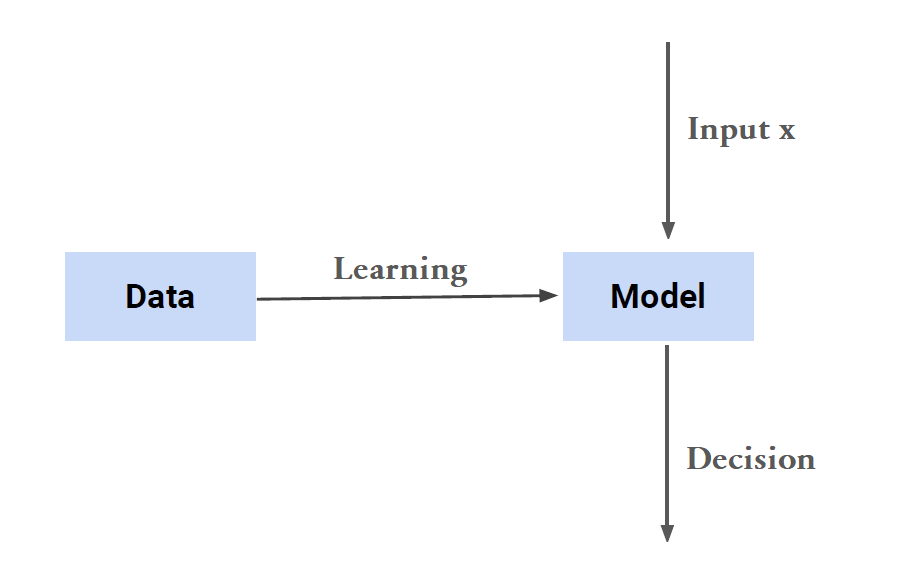
\includegraphics[width=0.9\linewidth]{figure/ml_decision_process.png}
	\end{center}
\end{minipage}
}
\end{vbframe}

\begin{vbframe}{Decision Theory 101}
	%	
	\scriptsize{
		%
		%
		\begin{itemize}
%			
			\item In binary classification, we typically call one class "positive" and the 
			other "negative".
%			
			\item The positive class is the more important, often smaller one.
%			
			\item The confusion matrix gives an overview over the errors as well as correct decisions in a tabulated form:
%
		\end{itemize}
		
		\begin{center}
			\footnotesize
			\begin{tabular}{cc|>{\centering\arraybackslash}p{7em}>{\centering\arraybackslash}p{8em}}
				& & \multicolumn{2}{c}{\bfseries True Class $y$} \\
				& & $+$ & $-$ \\
				\hline
				\bfseries Decision     & $+$ & True Positive (TP)  & False Positive (FP) \\
				$\yh$ & $-$ & False Negative (FN) & True Negative (TN) \\
			\end{tabular}
		\end{center}
		% \\
		Here:
		\begin{itemize}
%			\footnotesize
			\item \textbf{True Positive} (TP) means that we decide for +1 for a given instance 
			that is really a +1 (correct decision).
			 \item \textbf{False Positive} (FP) means that we decide for +1 for a given instance 
			 that is actually a -1 (incorrect decision). 
			\item \textbf{False Negative} (FN) means that we decide for -1 for a given instance 
			that is actually a +1 (incorrect decision). 
			 \item \textbf{True Negative} (TN) means that we decide for -1 for a given instance 
			 that is really a -1 (correct decision).
		\end{itemize}
		
		%
	}
\end{vbframe}


\begin{vbframe}{Decision Theory 101}
%	
\scriptsize{
%	
	The confusion matrix gives rise to common classification/decision criteria, which highlight different aspects
	of the decision making.
%	
	\begin{center}
		\footnotesize
		\renewcommand{\arraystretch}{1.1}
		\begin{tabular}{cc||cc|c}
			& & \multicolumn{2}{c|}{\bfseries True Class $y$} & \\
			& & $+$ & $-$ & \\ 
			\hline \hline
			\bfseries Decision     & $+$ & TP & FP & $\rho_{PPV} = \frac{\text{TP}}{\text{TP} + \text{FP}}$\\
			$\yh$ & $-$ & FN & TN & $\rho_{NPV} = \frac{\text{TN}}{\text{FN} + \text{TN}}$\\
			\hline
			& & $\rho_{TPR} = \frac{\text{TP}}{\text{TP} + \text{FN}}$ & $\rho_{TNR} = \frac{\text{TN}}{\text{FP} + \text{TN}}$ & $\rho_{ACC} = \frac{\text{TP}+ \text{TN}}{\text{TOTAL}}$
		\end{tabular}
		\renewcommand{\arraystretch}{1}
	\end{center}
%	
	\begin{itemize}
%		
		\item True positive rate $\rho_{TPR}$: for how many of the true 1s did we decide for 1?
%		
		\item [$\leadsto$] Population counterpart: $\P (\yh =1 ~|~ y=1)$
%		
		\item True Negative rate $\rho_{TNR}$: for how many of the true -1s did we decide for -1?
%		
		\item [$\leadsto$] Population counterpart: $\P (\yh = -1 ~|~ y= -1)$
%		
		\item Positive predictive value $\rho_{PPV}$: if we decide for 1, how likely is 
		it a true 1?
%		
		\item [$\leadsto$] Population counterpart: $\P (y = 1 ~|~ \yh = 1)$
%		
		\item Negative predictive value $\rho_{NPV}$: if we decide for -1, how likely is 
		it a true -1?
%		
		\item [$\leadsto$] Population counterpart: $\P (y = -1 ~|~ \yh = -1)$
%
		\item Accuracy $\rho_{ACC}$: for how many instances did we decide correctly?
%		
		\item [$\leadsto$] Population counterpart: $\P (\yh = y  )$
	\end{itemize}
}
\end{vbframe}


\begin{vbframe}{Decision Theory 101}
	%	
	\footnotesize{
		%	
		The confusion matrix gives rise to common classification/decision criteria, which highlight different aspects
		of the decision making
		%	
		\begin{center}
			\footnotesize
			\renewcommand{\arraystretch}{1.1}
			\begin{tabular}{cc||cc|c}
				& & \multicolumn{2}{c|}{\bfseries True Class $y$} & \\
				& & $+$ & $-$ & \\ 
				\hline \hline
				\bfseries Decision     & $+$ & TP & FP & $\rho_{PPV} = \frac{\text{TP}}{\text{TP} + \text{FP}}$\\
				$\yh$ & $-$ & FN & TN & $\rho_{NPV} = \frac{\text{TN}}{\text{FN} + \text{TN}}$\\
				\hline
				& & $\rho_{TPR} = \frac{\text{TP}}{\text{TP} + \text{FN}}$ & $\rho_{TNR} = \frac{\text{TN}}{\text{FP} + \text{TN}}$ & $\rho_{ACC} = \frac{\text{TP}+ \text{TN}}{\text{TOTAL}}$
			\end{tabular}
			\renewcommand{\arraystretch}{1}
		\end{center}
		%	
		\begin{itemize}
			%		
			\item False positive rate $\rho_{FPR} = \frac{\text{FP}}{\text{FP} + \text{TN}}$: for how many of the true -1s did we decide for +1?
			%		
			\item [$\leadsto$] Population counterpart: $\P (\yh = +1 ~|~ y= -1)$
			%		
			\item False Negative rate $\rho_{FNR} = \frac{\text{FN}}{\text{TP} + \text{FN}}$: for how many of the true 1s did we decide for -1?
			%		
			\item [$\leadsto$] Population counterpart: $\P (\yh = -1 ~|~ y= 1)$
			%		
			\item Error $\rho_{err} = 1- \rho_{ACC}$ for how many instances did we decide incorrectly?
			%		
			\item [$\leadsto$] Population counterpart:  $\P (\yh \neq y  )$
			%		
		\end{itemize}
	}
\end{vbframe}


\begin{vbframe}{Sensitive attributes/features}
	%	
	\small{
		%	
		\begin{itemize}
%			
			\item The aspect of fairness usually arises due to the presence of sensitive attributes/features among the attributes/features  $\xv_1, \ldots, \xv_p,$ e.g.\ age, gender, nationality, race, $\ldots$
%			
			\item Note that we assume that the attribute/feature observations $\xv^{(1)},\ldots,\xv^{(n)}$ are random observations of the random vector $\xv=(x_1,\ldots,x_p)^\top$ with distribution $\Px.$ Accordingly, the j-th attribute/feature vector $\xj = \xjvec$ is a collection of random observations of the random variable $x_j$ with distribution $\Pxj,$ which is the marginal distribution of $\Px$ for the j-th attribute/feature.
%
			\item We introduce the random variable $\sens$ to capture all sensitive attributes/features, which typically has discrete values.
%			
			\item The basic idea of fairness criteria introduced for machine learning methods is to equalize different decision criteria or statistical quantities  involving $\sens$.
%			

			\scriptsize{This goes back to Anne Clearly in the 1960s who studied group differences in educational testing.}
%			
		\end{itemize}
	}
\end{vbframe}


\begin{frame}{Removing sensitive features}
	%	
	\small{
		%	
		\begin{itemize}
			%			
			\item A straightforward (and also naive) approach is to simply ignore or remove all sensitive features at prediction time. This approach is often called \emph{fairness through unawareness.}  However, in many cases other non-sensitive features are slightly correlated with the sensitive one(s). For example:
%			
			\begin{itemize}
				\small
%				
				\item gender with hobbies or interests (job application),
%				
				\item race and zip code (law systems),
%				
				\item nationality and location id (credit application),
%				
				\item $\ldots$
%				
			\end{itemize}
			%			
			\item Thus, an ML model trained on data including the sensitive features might combine the corresponding correlated non-sensitive features to make essentially the same decision, as it still seeks to maximize accuracy.
			%			
			\begin{center}
				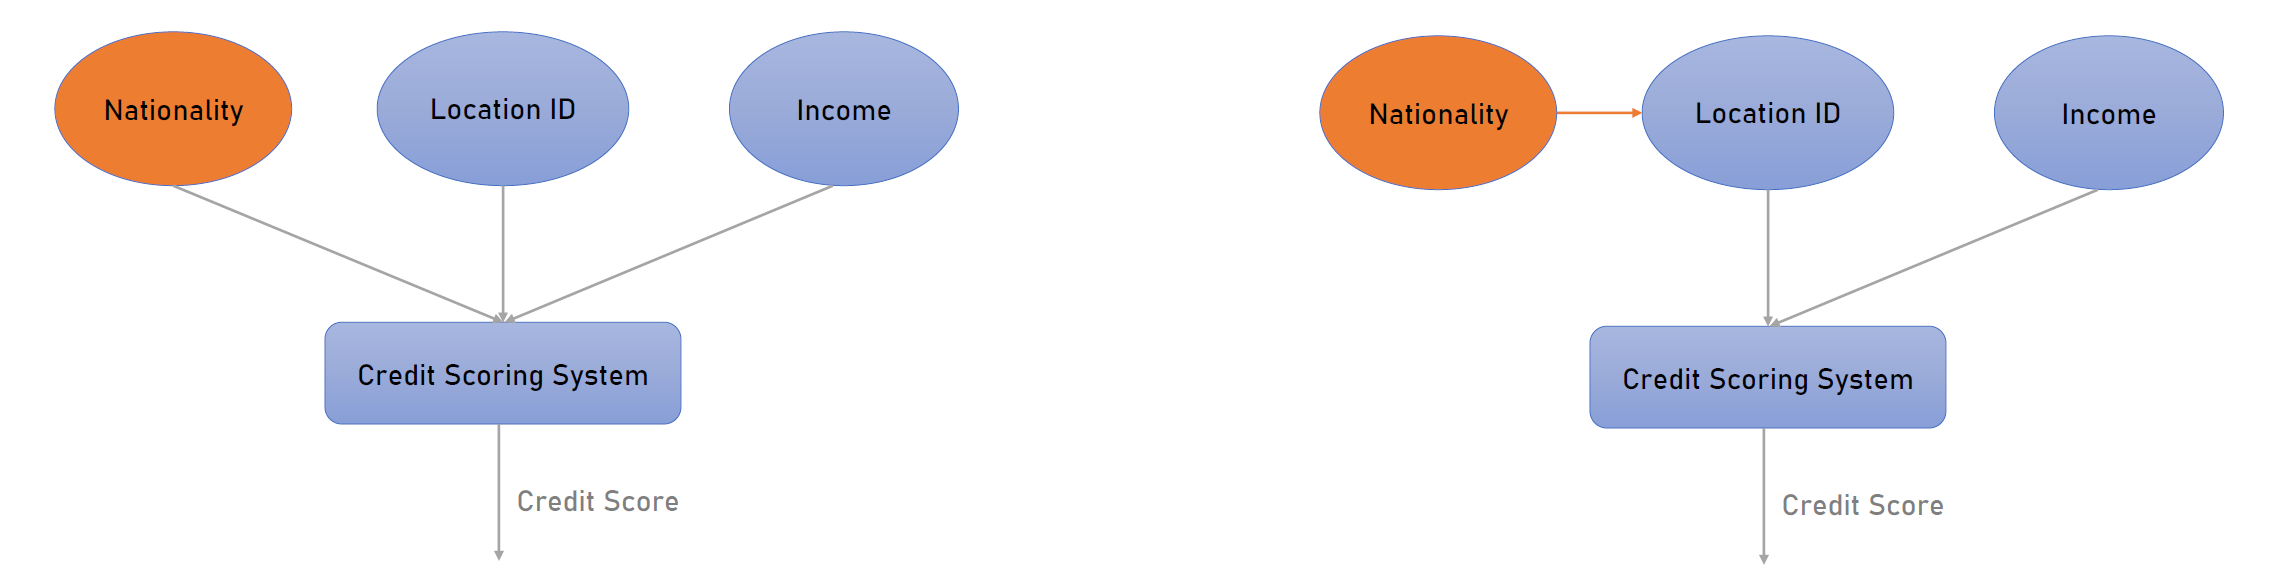
\includegraphics[width=0.7\linewidth]{figure/fair_unaware}
			\end{center}
		\end{itemize}
	}
\end{frame}

\begin{vbframe}{Independence as a Fairness Criterion}
	%	
	\small{
		%	
		\begin{itemize}
			%			
			\item A quite natural fairness criterion is given by ensuring (stochastic) independence between the decision $\yh$ and the sensitive attributes/features $\sens:$
%			
			$$	\yh \indep \sens	$$
%			
			\item This is equivalent to ensuring an equal ``acceptance rate'' among all possible realizations $\ba,\batilde$ of $\sens:$
%			
			$$  \P(  \yh = 1 ~|~ \sens = \ba ) = \P(  \yh = 1 ~|~ \sens = \batilde )$$
			%			
			\item This criterion is also known as statistical/demographic parity, group fairness, equal positive rates or Darlington's fourth criterion.
%			
			\item One can relax the criterion by introducing a fixed tolerance parameter $\eps>0$ and only require that for all possible realizations $\ba,\batilde$ of $\sens$ it holds that
%			
			$$  \big|  \P(  \yh = 1 ~|~ \sens = \ba ) - \P(  \yh = 1 ~|~ \sens = \batilde ) \big| \leq \eps $$
%		
		\end{itemize}
%	
	}
\end{vbframe}


\begin{vbframe}{Downsides of Independence as a Fairness Criterion}
	%	
	\small{
		%	
		\begin{itemize}
			%			
			\item Independence does not take into account that the outcome $y$ might be correlated with $\sens,$ which means that the different realizations of $\sens$ have different underlying distributions for $y.$
			%			
			\item Not considering this dependency can lead to decisions which are fair trough the lens of the independence criterion, but not for the groups themselves. 
%			
			\item Moreover, independence does not rule out the possibility of unfair practices. For example, consider a job hiring process involving different groups of people. Assume that we 
%			
			\begin{itemize}
				\small
%				
				\item make thoughtful and good decisions in one specific group with accepting people from that group with a rate $p\in(0,1),$
%				
				\item make poor and bad decisions in all other groups with the same acceptance rate $p\in(0,1),$ respectively.
%							
			\end{itemize}	
%		
		\end{itemize}
		%	
	}
\end{vbframe}


\begin{vbframe}{Achieving Independence via Representation Learning}
	%	
	\small{
		%	
		\begin{itemize}
			%		
			\begin{minipage}{0.5\textwidth}	
%				
			\item One common idea to satisfy the independence criterion is by finding a ``fair representation'' $\mathbf{Z}$ of the data $\xv,$ i.e., one such that $ \mathbf{Z} \indep \sens$ holds.
%			
			Then, the ML method $f$ uses $\mathbf{Z}$ instead of $\xv$ for the decision: $\yh = f(\mathbf{Z})$
%			
			\end{minipage}
			\begin{minipage}{0.4\textwidth}
				\centering
				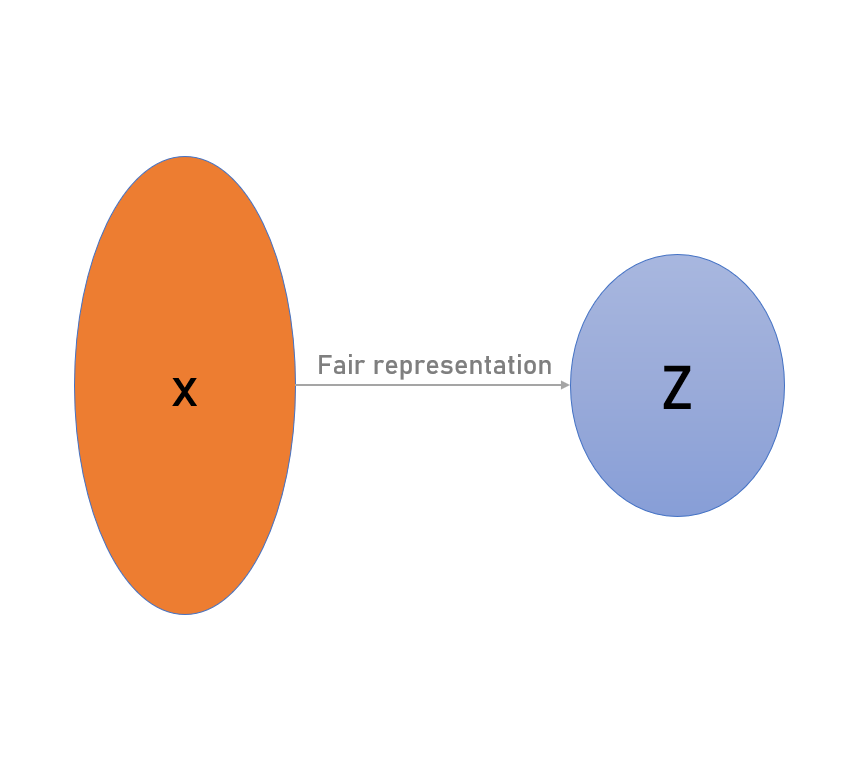
\includegraphics[width=0.8\linewidth]{figure/fair_representation.png}
			\end{minipage}
			%			
			\item The idea goes back to Zernel et al. (2013), where three requirements on the representation are formulated:
%			
			\begin{enumerate}
				\small
%				
				\item Information about $\xv$ should be preserved $\Leftrightarrow$ Mutual information between $\xv$ and $\mathbf{Z}$ is high.
%				
				\item The sensitive attributes/features $\sens$ are obfuscated $\Leftrightarrow$ Mutual information between $\sens$ and $\mathbf{Z}$ is low.
%				
				\item Accuracy of the model $f$ using $\mathbf{Z}$ is (still) high $\Leftrightarrow$ Mutual information between $y$ and $\mathbf{Z}$ is high.
%				
			\end{enumerate}
			%			
%			\item 
%			
		\end{itemize}
		%	
	}
\end{vbframe}


\begin{vbframe}{Separation as a Fairness Criterion}
	%	
	\footnotesize{
		%	
		\begin{itemize}
			%			
			\item As we discussed above, the independence criterion does not take correlation between $y$ and $\sens$ into account. As an alternative fairness criterion one can consider \emph{separation,} which ensures (stochastic) independence between the decision $\yh$ and the sensitive attributes $\sens$ given $y:$
			%			
			$$	\yh \indep \sens ~|~y	$$
			%			
			\item This is equivalent to equalize the (population) error rates for all possible realizations $\ba,\batilde$ of $\sens:$
			%			
			\begin{align*}
				 &\P(  \yh = 1 ~|~ y = -1, \sens = \ba ) = \P(  \yh = 1 ~|~ y=-1, \sens = \batilde ) \tag{equal false positive rates}\\
				 &\P(  \yh = -1 ~|~ y = 1, \sens = \ba ) = \P(  \yh = -1 ~|~ y=1, \sens = \batilde ) \tag{equal false negative rates}
			\end{align*}
			%		
			\item The idea is that all realizations of $\sens$ experience the same FPR and FNR.
%				
			\item This criterion is also known as equalized odds, avoiding disparate mistreatment, equalized error rates or conditional procedure accuracy.
%			
			\item This is a posthoc criterion, as it is not known at the time of the decision whether the current instance is positive or negative. Only in hindsight the positive and negative instances can be collected and compared with the decisions made. 
			%			
		\end{itemize}
		%	
	}
\end{vbframe}



\begin{vbframe}{Interlude: ROC Space}
	
	\begin{itemize}
		\item For comparing classifiers, we characterize them by their TPR and FPR values and plot them in 
		a coordinate system.
		\item We could also use two different ROC metrics (decision criteria) which define a trade-off, 
		for instance, TPR and PPV.
	\end{itemize}
	
	\lz
	
	\begin{minipage}[c]{0.5\textwidth}
		\begin{knitrout}
			\scriptsize
			\definecolor{shadecolor}{rgb}{0.969, 0.969, 0.969}\color{fgcolor}
			{\centering 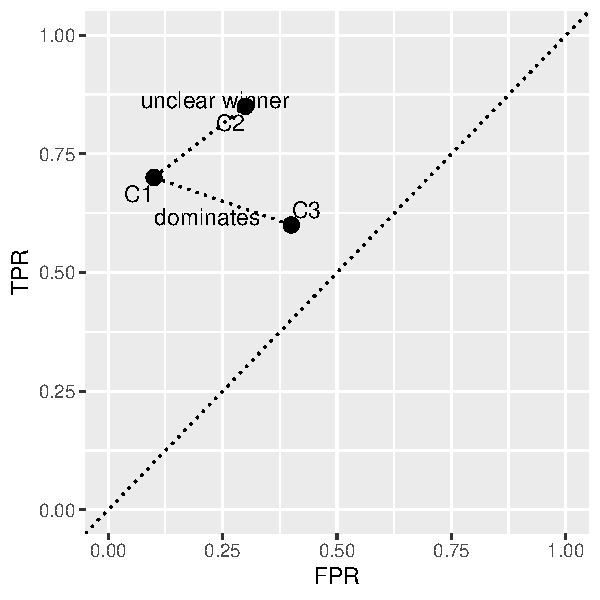
\includegraphics[width=\textwidth]{figure/eval_mclass_roc_sp_1}}
		\end{knitrout}
	\end{minipage}%
	\begin{minipage}[c]{0.5\textwidth}
		% 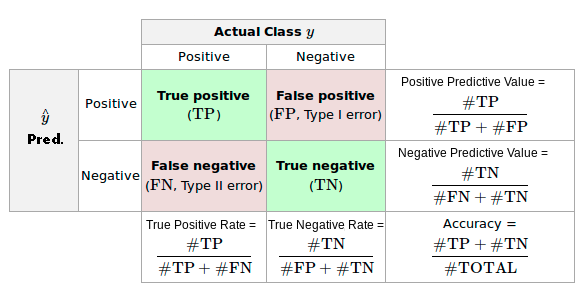
\includegraphics[width=\textwidth]{figure_man/roc-confmatrix2.png}
		\begin{center}
			\small
			\begin{tabular}{cc|cc}
				& & \multicolumn{2}{c}{\bfseries True Class $y$} \\
				& & $+$ & $-$ \\
				\hline
				\bfseries Pred.     & $+$ & TP & FP \\
				$\yh$ & $-$ & FN & TN \\
			\end{tabular}
			\lz
			$$\text{TPR} = \frac{\text{TP}}{\text{TP} + \text{FN}}$$
			$$\text{FPR} = \frac{\text{FP}}{\text{FP} + \text{TN}}$$
		\end{center}
	\end{minipage}
	
\end{vbframe}



\begin{vbframe}{Interlude: ROC Space}
	
	\begin{itemize}
		\item The best classifier lies on the top-left corner, where FPR equals 0 and 
		TPR is maximal.
		\item The diagonal is worst as it corresponds to a classifier producing random 
		labels (with different proportions). 
	\end{itemize}
	
	\lz
	
	\begin{minipage}[c]{0.5\textwidth}
		\begin{itemize}
			\item If each positive $x$ will be randomly classified 
			with 25\% as "pos", $\text{TPR} = 0.25$.
			\item If we assign each negative $x$ randomly to "pos", $\text{FPR} = 0.25$.

		\end{itemize}
	\end{minipage}%
	\begin{minipage}[c]{0.5\textwidth}
		\centering 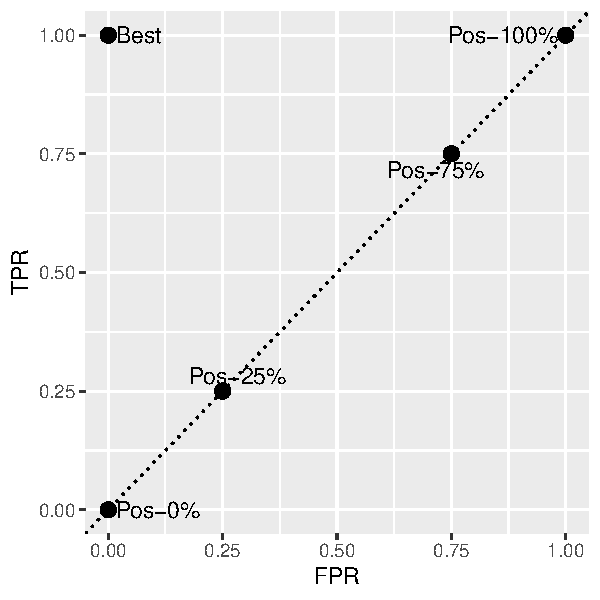
\includegraphics[width=0.8\textwidth]{figure/eval_mclass_roc_sp_2}
	\end{minipage}
	
\end{vbframe}



\begin{vbframe}{Interlude: ROC Curves for scoring classifiers}
	\small
	\begin{itemize}
%		
		\item 	Many binary classification methods use a score (function) $s:\Xspace \to \R$ and a threshold value $c$ to make the prediction (decision):
		%	
		$$\fx = 2 \cdot \mathds{1}_{[ s(\xv) \ge c]} -1.$$
		%	
		\item The choice of threshold affects the TPR and FPR, so it is interesting to examine the effects of different thresholds on these.
		
		\item A ROC curve is a visual tool to help in finding good threshold values.
%		
	\end{itemize}
	
	\framebreak
	
%	A common measure of predictiveness is the area under the curve, which is the probability that a random positive instance gets a score higher than a random negative instance. An area of 1/2 corresponds to random 	guessing, and an area of 1 corresponds to perfect classification, or 	more formally, the score equals the target.
	
	\textbf{To draw a ROC curve}:
	
	(W.l.o.g.\ $s:\Xspace \to [0,1]$)
	
	\lz
	
	\begin{minipage}[b]{0.65\textwidth}
		\small
		\begin{enumerate}
			\item Rank test observations on decreasing score.
			\item Start with $c = 1$, so we start in $(0, 0)$; we predict everything as
			negative.
			\item Iterate through all possible thresholds $c$ and proceed for each
			observation $x$ as follows:
			\begin{itemize}
				\footnotesize
				\item If $x$ is positive, move TPR $1/n_+$ up, \\as we have one TP more.
				\item If $x$ is negative, move FPR $1/n_-$ right, \\as we have one FP  more.
%				\item (Make a diagonal move in case of ties)
			\end{itemize}
		\end{enumerate}
	\end{minipage}%
	\begin{minipage}[b]{0.35\textwidth}
		\centering
		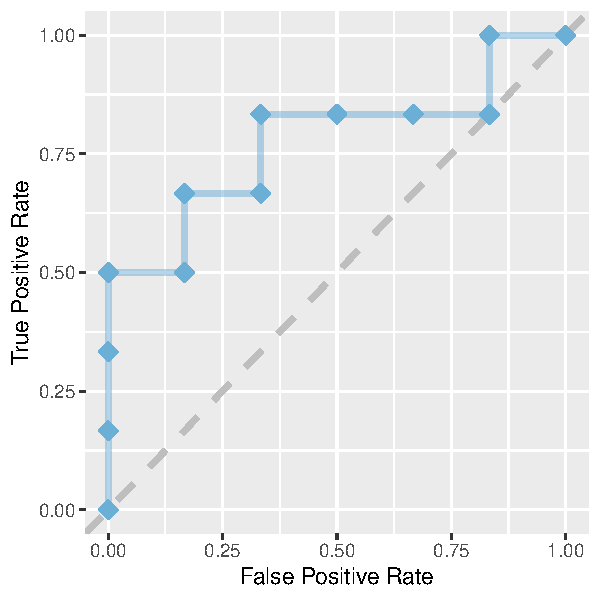
\includegraphics[width=\textwidth]{figure/eval_mclass_roc_sp_4}
	\end{minipage}
	
	\scriptsize($n_+:$ number of positives, $n_-:$ number of negatives.)
\end{vbframe}


% ------------------------------------------------------------------------------

\begin{vbframe}{Drawing ROC Curves: Example}
	
	% new frame for every animation step (rather than framebreak) to prevent plots
	% from jumping
	
	\begin{knitrout}\scriptsize
		\definecolor{shadecolor}{rgb}{0.969, 0.969, 0.969}\color{fgcolor}
		
		{
			% \centering 
			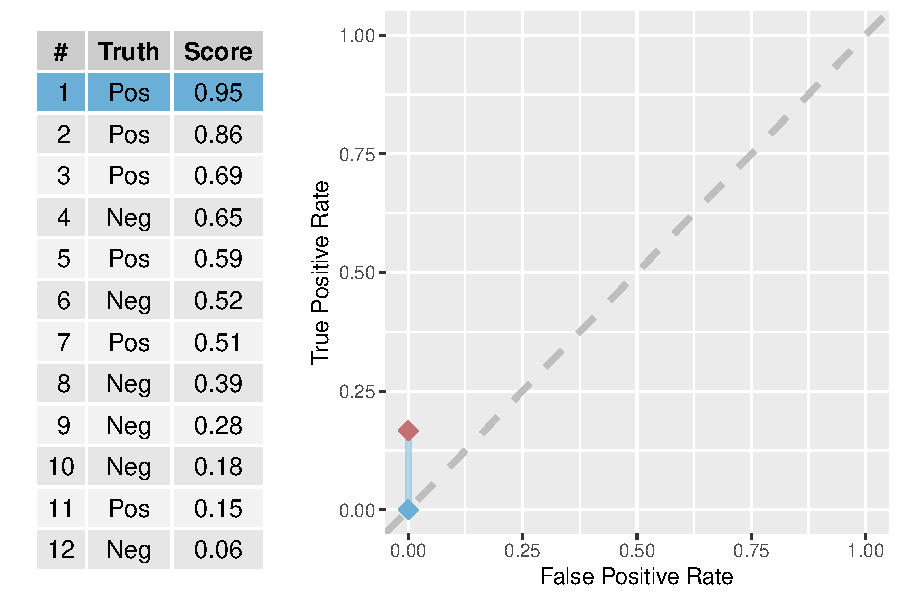
\includegraphics[width=0.8\textwidth]{figure/eval_mclass_roc_sp_5} 
		}
		
	\end{knitrout}
	
	\vfill
	
	\begin{minipage}[b]{0.3\textwidth}
		$c =$ 0.9\\ 
		$\rightarrow$ TPR = 0.167 \\
		$\rightarrow$ FPR = 0
	\end{minipage}%
	\begin{minipage}[b]{0.7\textwidth}
		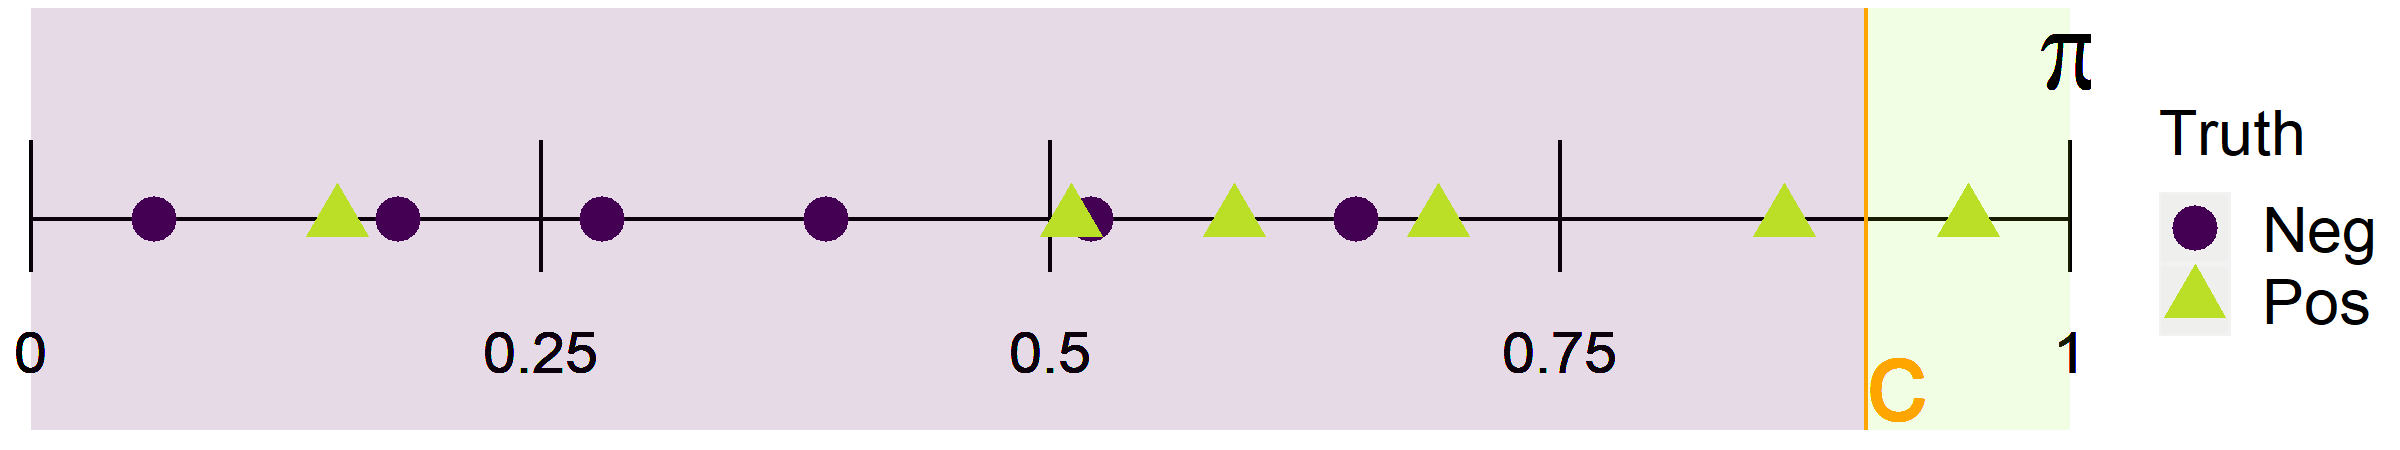
\includegraphics{figure/roc_horizontal_step_1} 
	\end{minipage}
	
\end{vbframe}

% ------------------------------------------------------------------------------

\begin{vbframe}{Drawing ROC Curves: Example}
	
	\begin{knitrout}\scriptsize
		\definecolor{shadecolor}{rgb}{0.969, 0.969, 0.969}\color{fgcolor}
		
		{
			% \centering 
			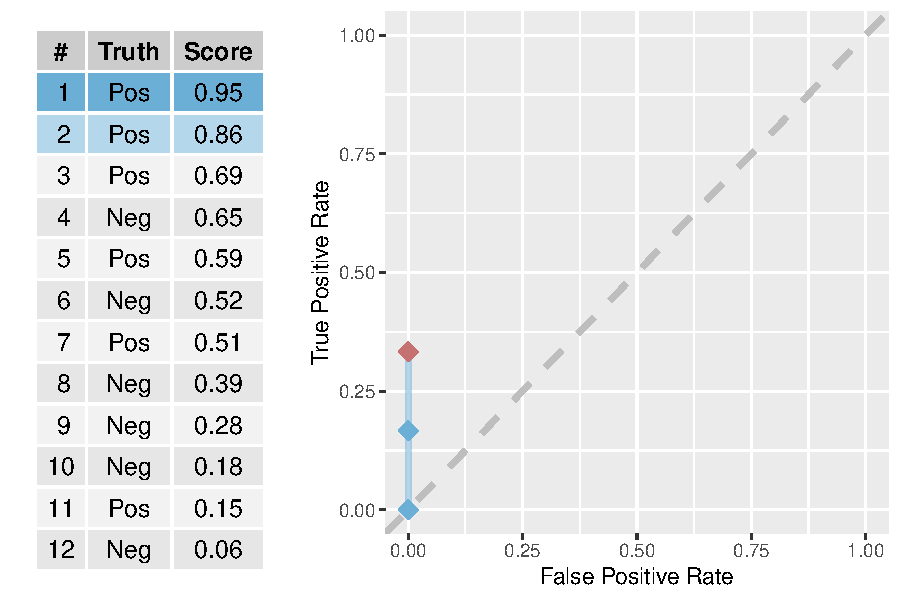
\includegraphics[width=0.8\textwidth]{figure/eval_mclass_roc_sp_6}
		}
		
	\end{knitrout}
	
	\vfill
	
	\begin{minipage}[b]{0.3\textwidth}
		$c =$ 0.85\\ 
		$\rightarrow$ TPR = 0.333 \\
		$\rightarrow$ FPR = 0
	\end{minipage}%
	\begin{minipage}[b]{0.7\textwidth}
		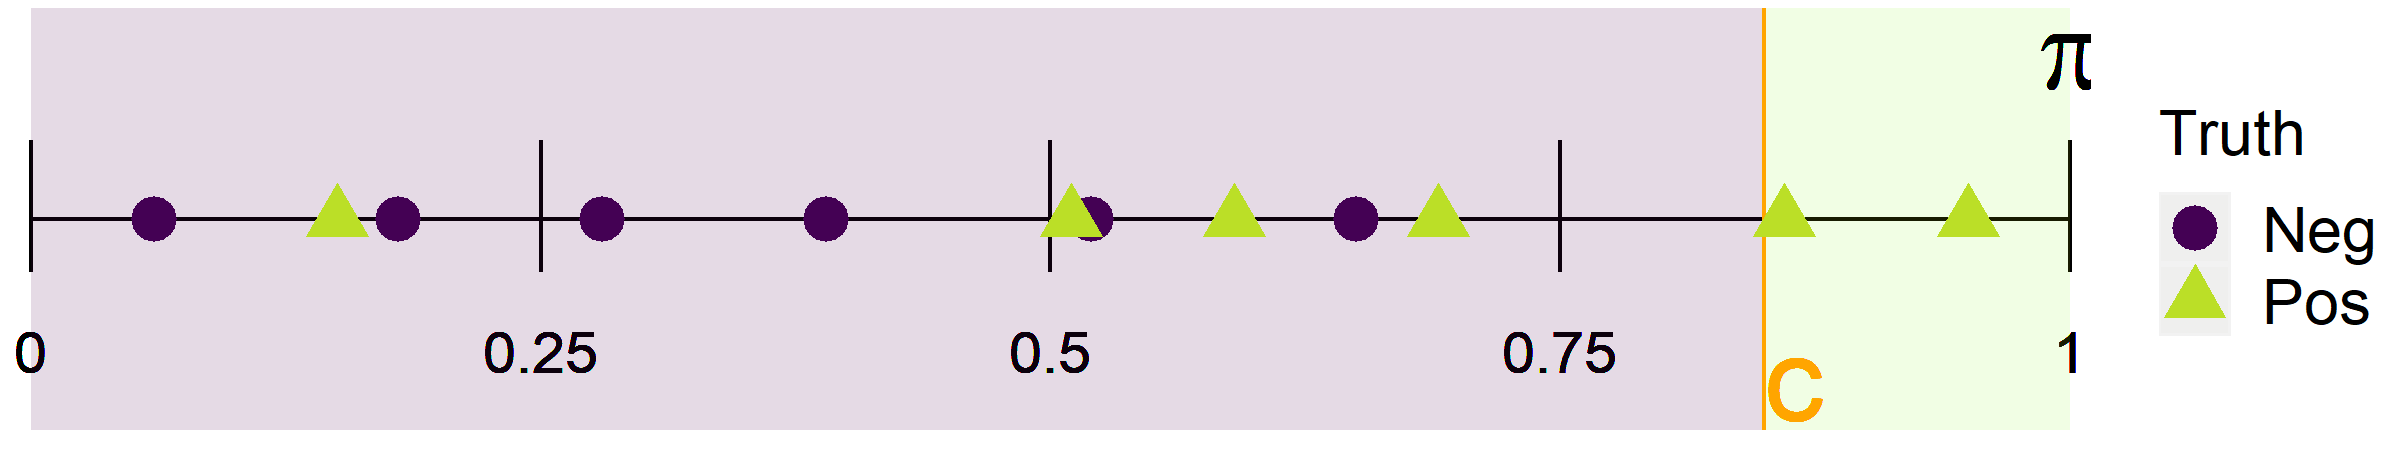
\includegraphics{figure/roc_horizontal_step_2} 
	\end{minipage}
	
\end{vbframe}

% ------------------------------------------------------------------------------

\begin{vbframe}{Drawing ROC Curves: Example}
	
	\begin{knitrout}\scriptsize
		\definecolor{shadecolor}{rgb}{0.969, 0.969, 0.969}\color{fgcolor}
		
		{
			% \centering 
			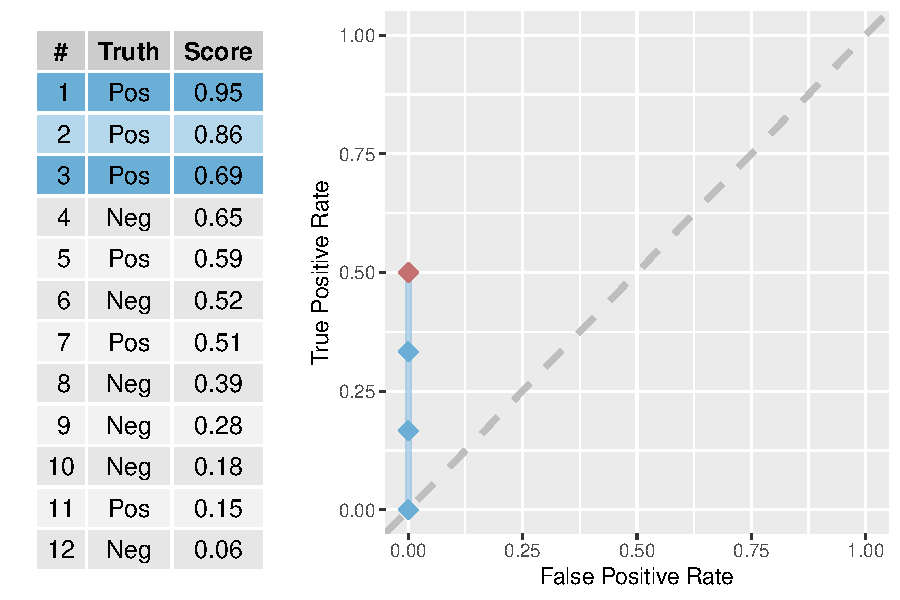
\includegraphics[width=0.8\textwidth]{figure/eval_mclass_roc_sp_7}
		}
		
	\end{knitrout}
	
	\vfill
	
	\begin{minipage}[b]{0.3\textwidth}
		$c =$ 0.66\\ 
		$\rightarrow$ TPR = 0.5 \\
		$\rightarrow$ FPR = 0
	\end{minipage}%
	\begin{minipage}[b]{0.7\textwidth}
		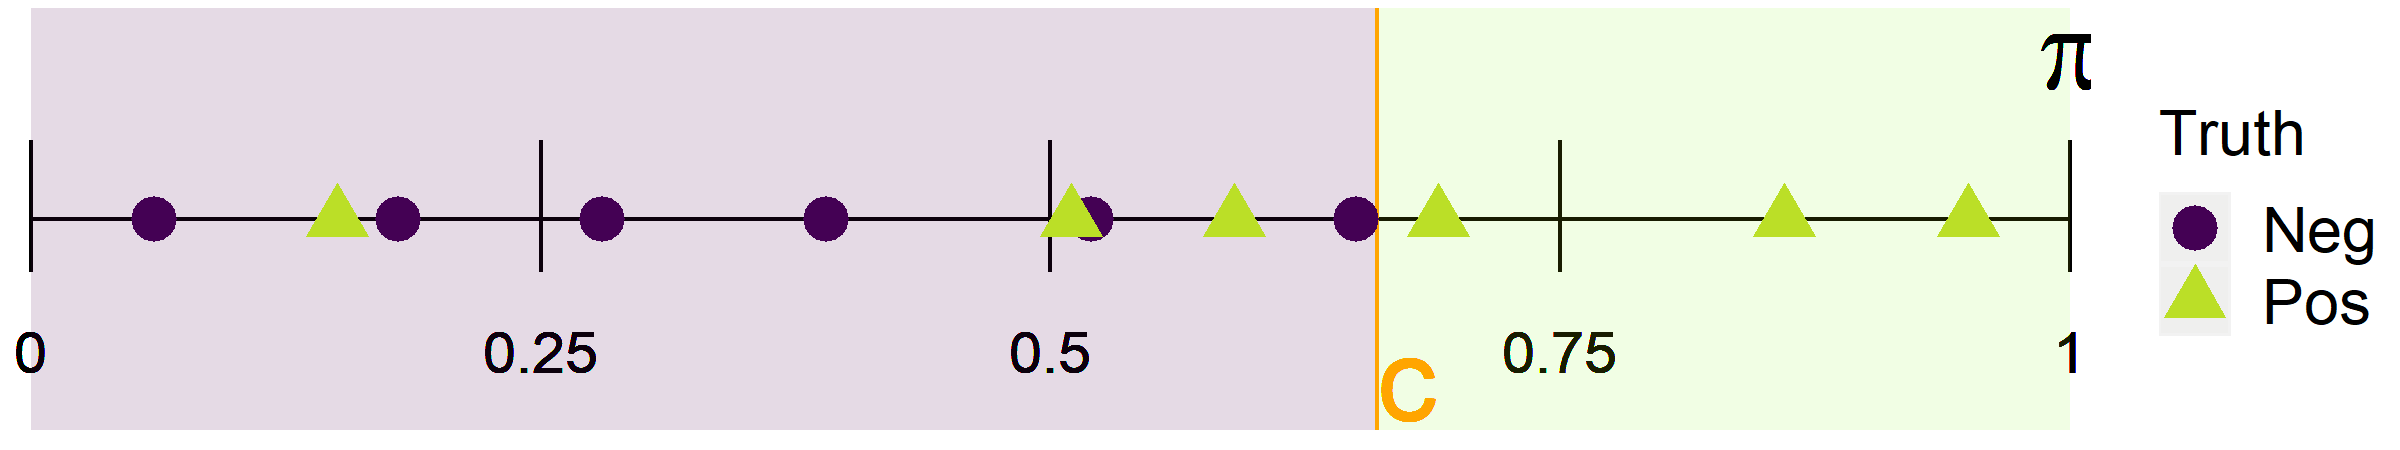
\includegraphics{figure/roc_horizontal_step_3} 
	\end{minipage}
	
\end{vbframe}

% ------------------------------------------------------------------------------

\begin{vbframe}{Drawing ROC Curves: Example}
	
	\begin{knitrout}\scriptsize
		\definecolor{shadecolor}{rgb}{0.969, 0.969, 0.969}\color{fgcolor}
		
		{
			% \centering 
			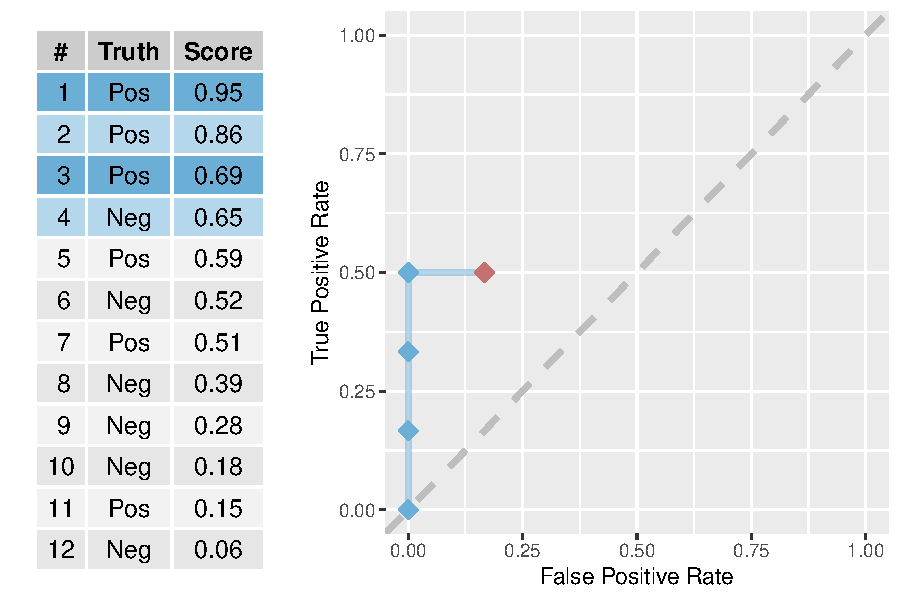
\includegraphics[width=0.8\textwidth]{figure/eval_mclass_roc_sp_8}
		}
		
	\end{knitrout}
	
	\vfill
	
	\begin{minipage}[b]{0.3\textwidth}
		$c =$ 0.6\\ 
		$\rightarrow$ TPR = 0.5 \\
		$\rightarrow$ FPR = 0.167
	\end{minipage}%
	\begin{minipage}[b]{0.7\textwidth}
		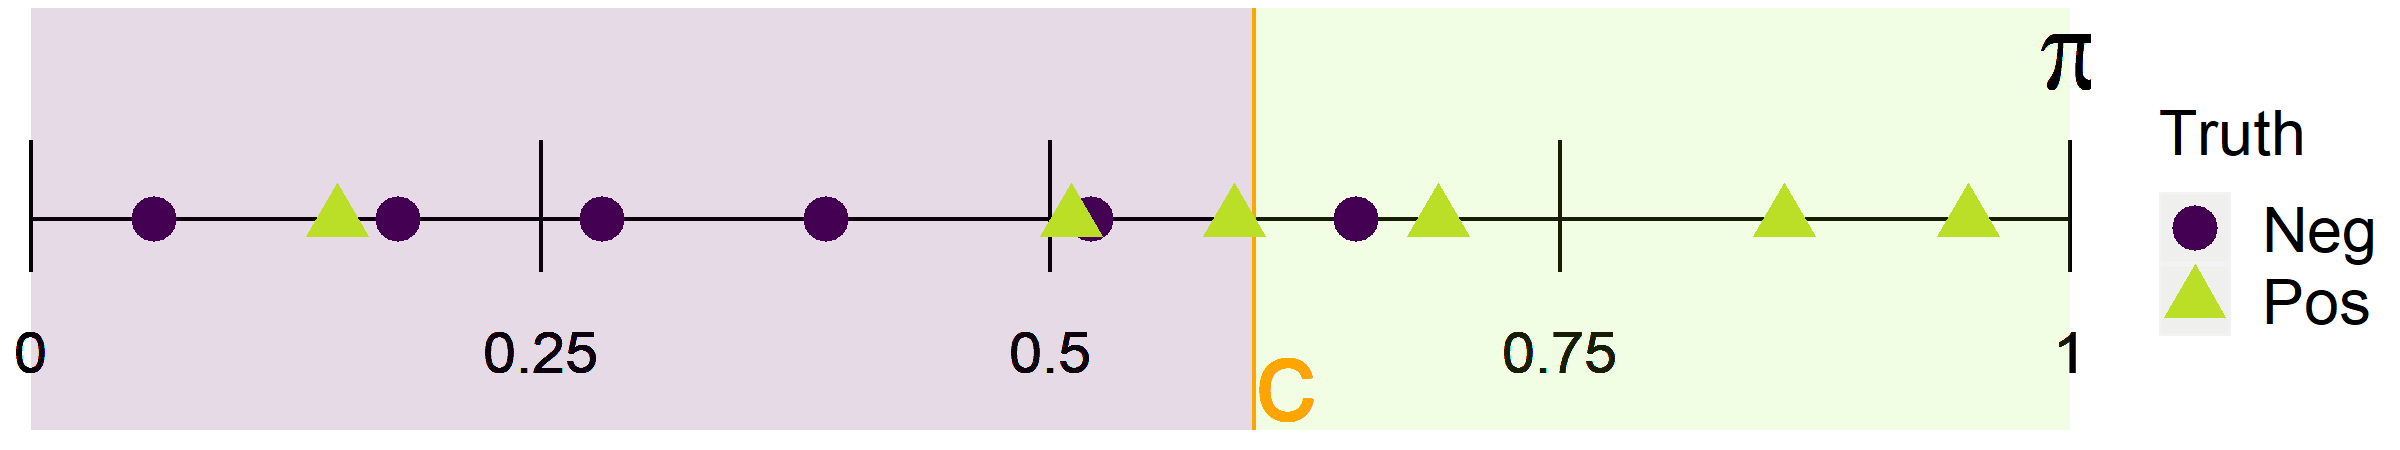
\includegraphics{figure/roc_horizontal_step_4} 
	\end{minipage}
	
\end{vbframe}

% ------------------------------------------------------------------------------

\begin{vbframe}{Drawing ROC Curves: Example}
	
	\begin{knitrout}\scriptsize
		\definecolor{shadecolor}{rgb}{0.969, 0.969, 0.969}\color{fgcolor}
		
		{
			% \centering 
			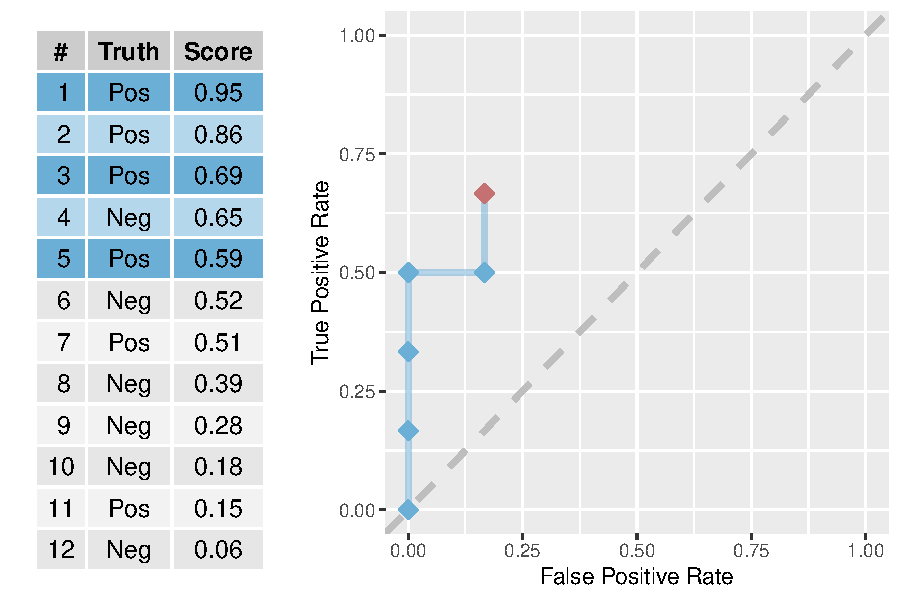
\includegraphics[width=0.8\textwidth]{figure/eval_mclass_roc_sp_9}
		}
		
	\end{knitrout}
	
	\vfill
	
	\begin{minipage}[b]{0.3\textwidth}
		$c =$ 0.55\\ 
		$\rightarrow$ TPR = 0.667 \\
		$\rightarrow$ FPR = 0.167
	\end{minipage}%
	\begin{minipage}[b]{0.7\textwidth}
		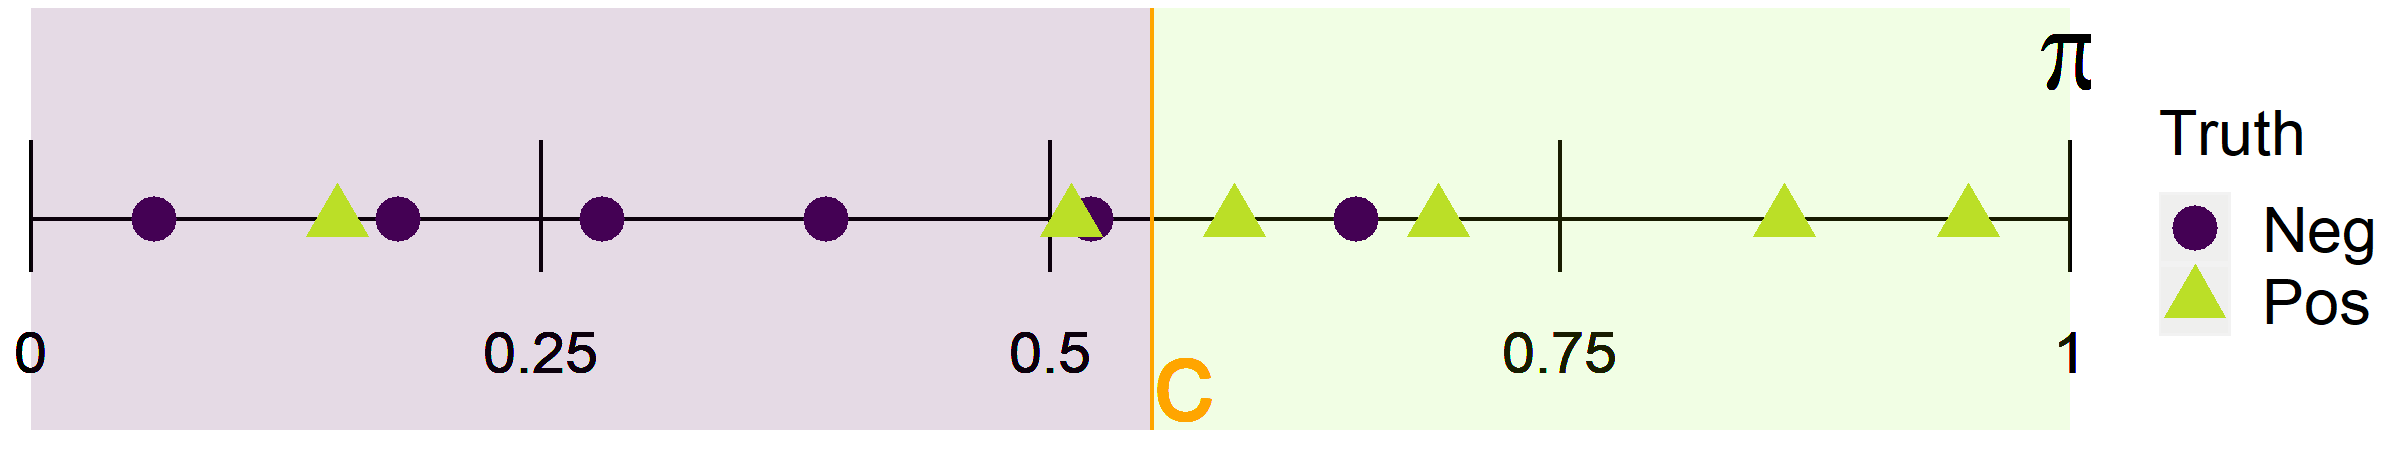
\includegraphics{figure/roc_horizontal_step_5} 
	\end{minipage}
	
\end{vbframe}

% ------------------------------------------------------------------------------

\begin{vbframe}{Drawing ROC Curves: Example}
	
	\begin{knitrout}\scriptsize
		\definecolor{shadecolor}{rgb}{0.969, 0.969, 0.969}\color{fgcolor}
		
		{
			% \centering 
			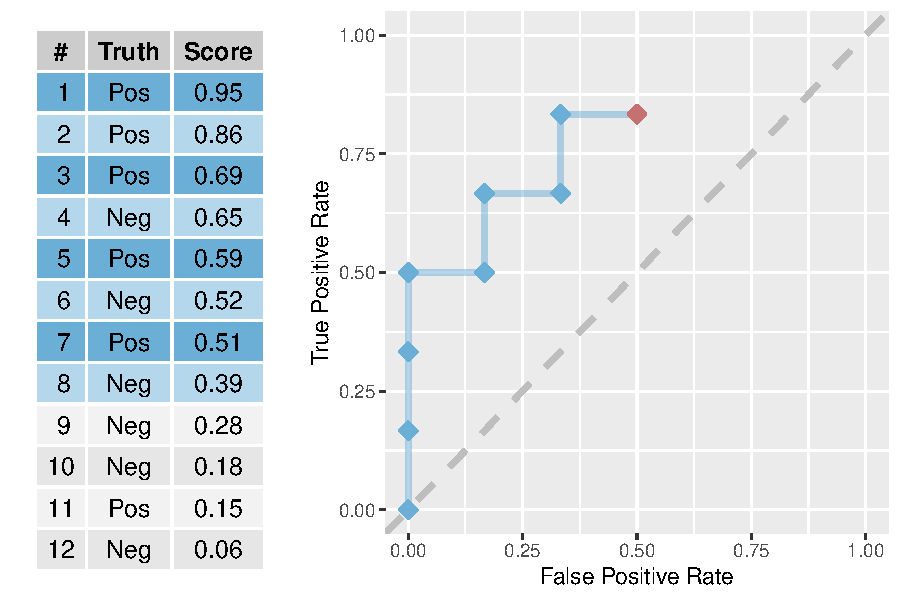
\includegraphics[width=0.8\textwidth]{figure/eval_mclass_roc_sp_10} 
		}
		
	\end{knitrout}
	
	\vfill
	
	\begin{minipage}[b]{0.3\textwidth}
		$c =$ 0.3\\ 
		$\rightarrow$ TPR = 0.833 \\
		$\rightarrow$ FPR = 0.5
	\end{minipage}%
	\begin{minipage}[b]{0.7\textwidth}
		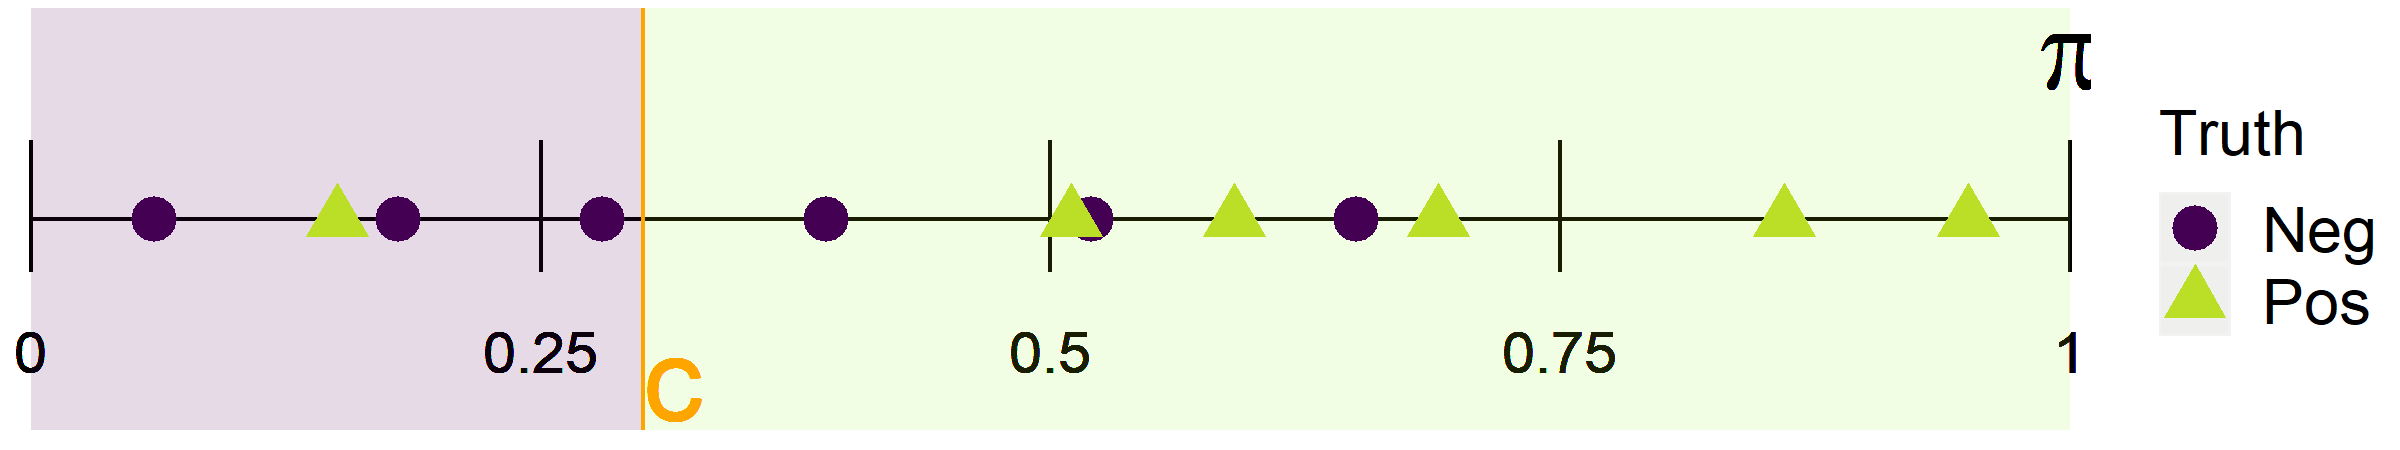
\includegraphics{figure/roc_horizontal_step_6} 
	\end{minipage}
	
\end{vbframe}

% ------------------------------------------------------------------------------

\begin{vbframe}{Drawing ROC Curves: Example}
	
	\begin{knitrout}\scriptsize
		\definecolor{shadecolor}{rgb}{0.969, 0.969, 0.969}\color{fgcolor}
		
		{
			% \centering 
			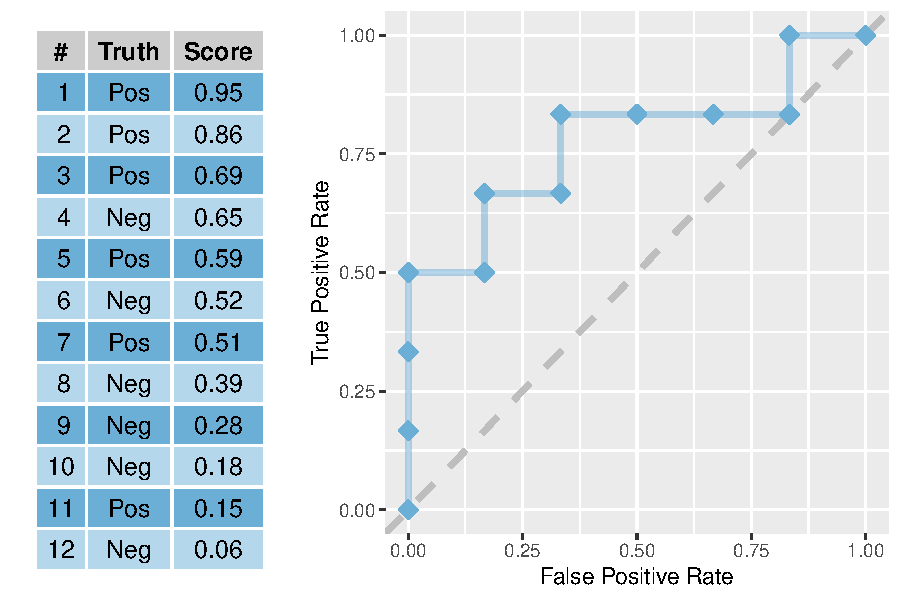
\includegraphics[width=0.8\textwidth]{figure/eval_mclass_roc_sp_11}
		}
		
	\end{knitrout}
	
	\vfill
	
	\begin{minipage}[b]{0.3\textwidth}
		$c =$ 0\\ 
		$\rightarrow$ TPR = 1 \\
		$\rightarrow$ FPR = 1
	\end{minipage}%
	\begin{minipage}[b]{0.7\textwidth}
		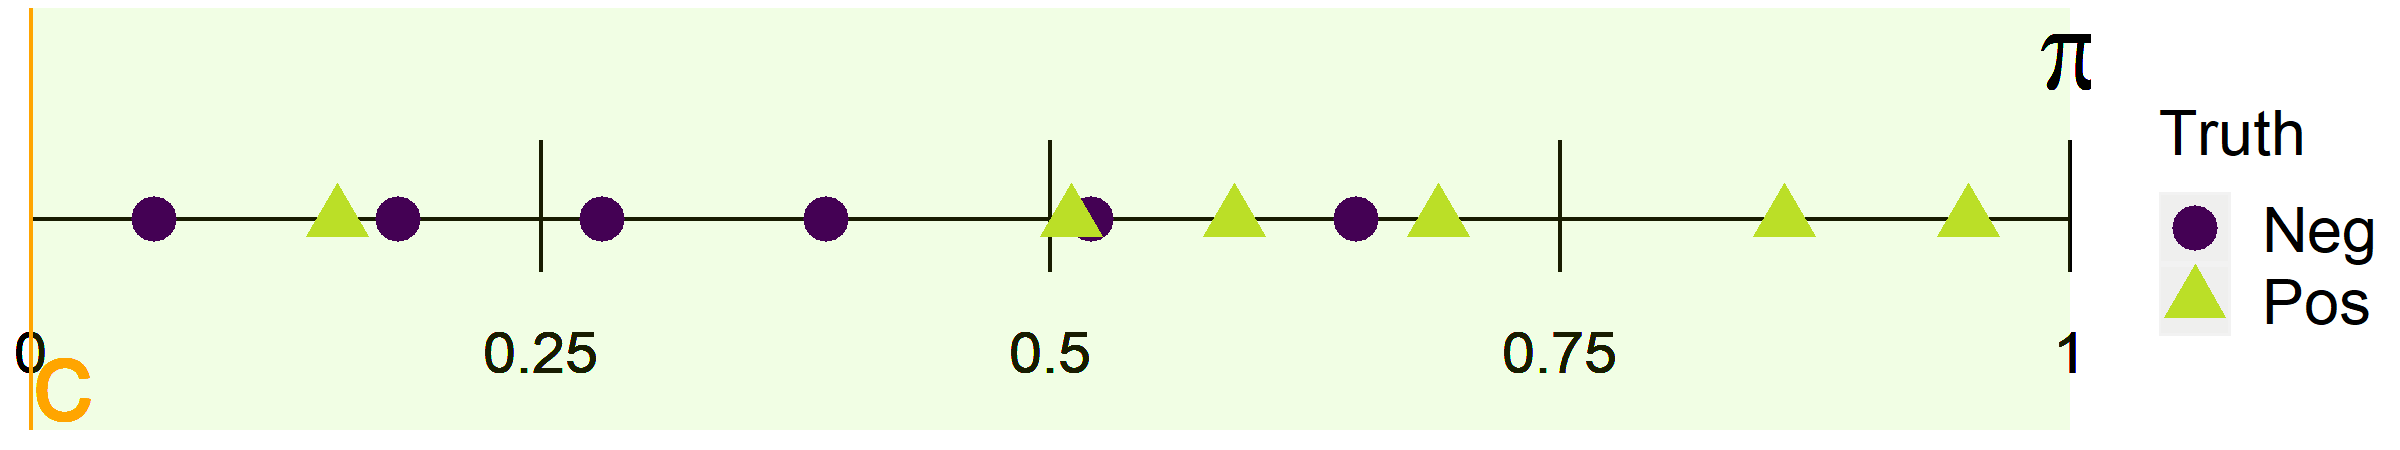
\includegraphics{figure/roc_horizontal_step_7} 
	\end{minipage}
	
\end{vbframe}

% ------------------------------------------------------------------------------

\begin{vbframe}{Separation and ROC Curves}
	%	
	\footnotesize{
		%	
		\begin{itemize}
			%			
			\item Separation, i.e.,
			%			
			\begin{align*}
				&\P(  \yh = 1 ~|~ y = -1, \sens = \ba ) = \P(  \yh = 1 ~|~ y=-1, \sens = \batilde ) \tag{equal FPRs}\\
				&\P(  \yh = -1 ~|~ y = 1, \sens = \ba ) = \P(  \yh = -1 ~|~ y=1, \sens = \batilde ) \tag{equal FNRs}
			\end{align*}
			%		
			means that all ROC curves of a classifier restricted on realizations of $\sens$ should be the same.
			%				
			This implies that the ROC curve of the score-based classifier conditional on realizations of $\sens$ must be
			``under'' all ROC curves.   
			%		
			
			\begin{center}
%				
				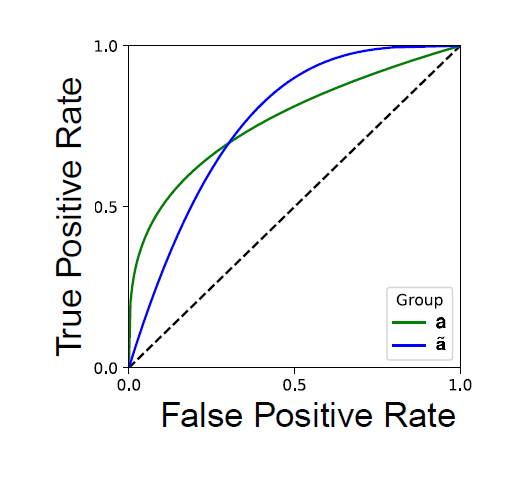
\includegraphics[width=0.3\textwidth]{figure/roc_curve_groups.png}
				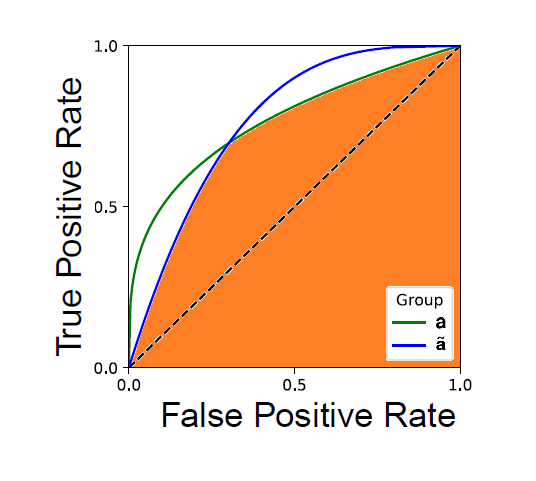
\includegraphics[width=0.3\textwidth]{figure/roc_curve_groups_area.png}
%				
			\end{center}
			
			\item In practice, we should never obtain a classifier below the diagonal.
%			
			\item Inverting the predicted labels ($-1 \mapsto 1$ and $1 \mapsto -1$) will 
			result in a reflection at the diagonal  $\Rightarrow \text{TPR}_{\text{new}} = 1 - \text{TPR}$ and 
			$\text{FPR}_{\text{new}} = 1 - \text{FPR}.$ \\	
		\end{itemize}
		%	
	}
\end{vbframe}

\begin{vbframe}{Downsides of Separation as a Fairness Criterion}
	%	
	\small{
		%	
		\begin{itemize}
			%			
			\item Consider two groups of people: blue and orange. We are interested to decide whether we should detain (positive class) a person and use a scoring classifier with scores in $[0,1]$ and a threshold $c=0.5.$
			
			\begin{center}
					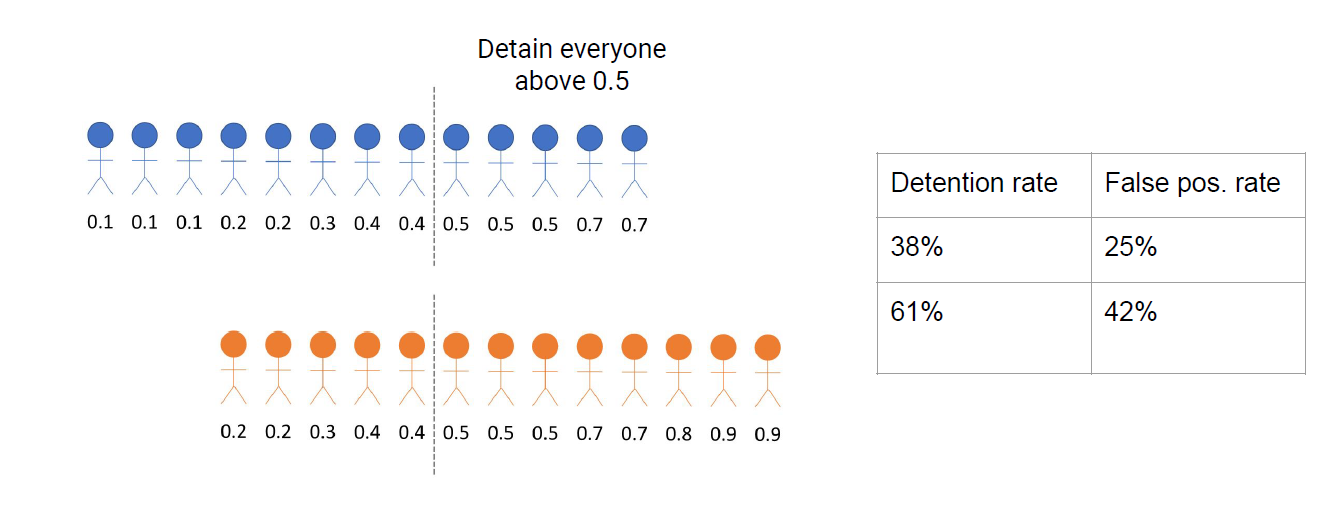
\includegraphics[width=0.8\textwidth]{figure/separation_issue_1.png}
			\end{center}  
			%			
			\item The classifier is not satisfying separation as FPR and FNR are not the same among the two groups.
			%			
			\framebreak
%			
			\item In order to achieve separation we would need to arrest more low risk individuals in the orange group.
			%			
			\begin{center}
				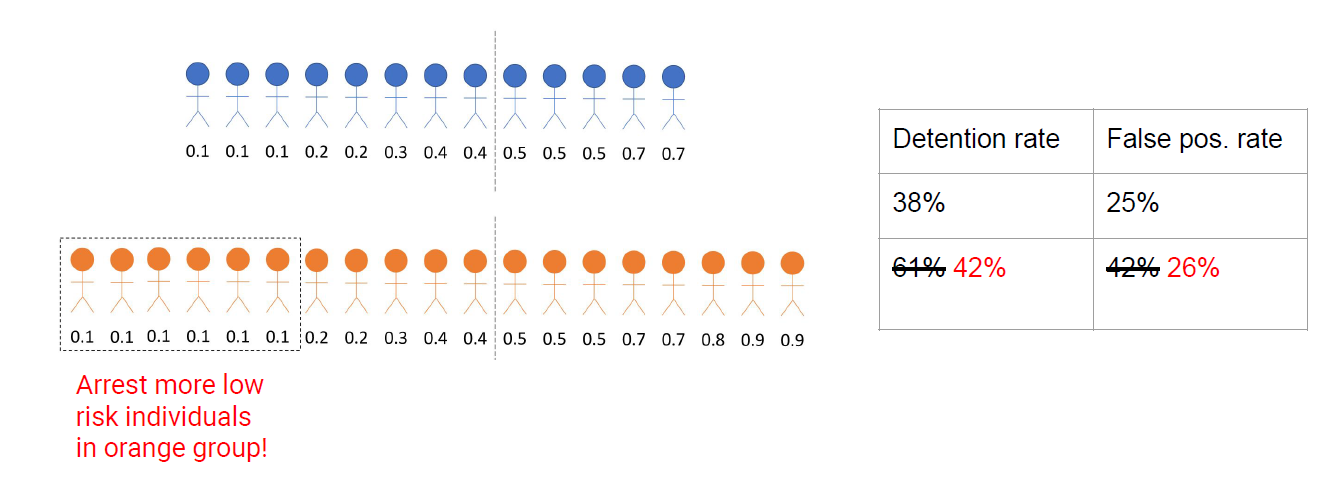
\includegraphics[width=0.9\textwidth]{figure/separation_issue_2.png}
			\end{center}
			%		
			\item Thus, as with achieving independence, separation can also lead to undesirable outcomes.
%			
		\end{itemize}
		%	
	}
\end{vbframe}


\begin{vbframe}{Sufficiency as a Fairness Criterion}
	%	
	\small{
		%	
		\begin{itemize}
			%			
			\item Another idea to specify a fairness criterion for score-based classifiers is that the corresponding score random variable $\mathbf{S} = s(\xv)$ already subsumes the sensitive attributes $\sens$ for the prediction: 
			%			
			$$	y \indep \sens ~|~ 	\mathbf{S}$$
%			
			%			
			\item This is equivalent to require that the fraction of positive instances assigned some score $s$ is the same for   all possible realizations $\ba,\batilde$ of $\sens:$
			%			
			\begin{align*}
				&\P(  y = 1 ~|~ \mathbf{S} = s, \sens = \ba ) = \P(  y = 1 ~|~  \mathbf{S} = s, \sens = \batilde ) 
			\end{align*}
			%				
			\item This criterion is also known as Cleary's model, conditional use accuracy or calibration within groups.
			%			
			\item This is an a priori guarantee: The decision maker sees the score value and knows based on this what the frequency of positives is.
			%			
		\end{itemize}
		%	
	}
\end{vbframe}



\begin{vbframe}{Sufficiency and Calibration}
	%	
	\footnotesize{
		%	
		\begin{itemize}
			%			
			\begin{minipage}{0.45\textwidth}
				\item Sufficiency is very closely related to the concept of \emph{calibration} of a probabilistic classifier, i.e., a classifier such that $s:\Xspace \to [0,1].$ More specifically, a probabilistic classifier is called \emph{calibrated} if for all $s\in[0,1]$
				%			
				$$  \P(  y = 1 ~|~ \mathbf{S} = s  ) = s. $$
			\end{minipage}
		\begin{minipage}{0.45\textwidth}
			\centering
			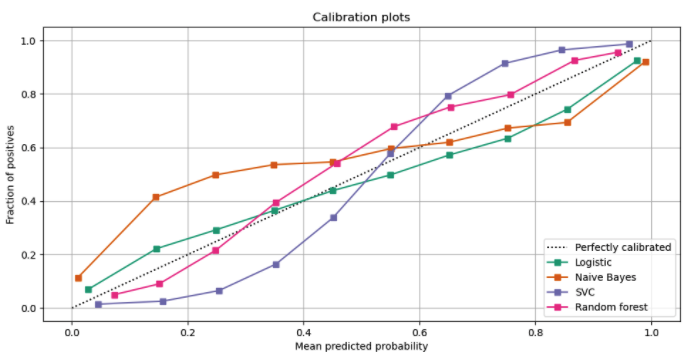
\includegraphics[width=0.9\textwidth]{figure/calibration.png}
		\end{minipage}
%			
			\item Note that: 
%			
			\begin{enumerate}
%				
			\footnotesize
%			
				\item This condition means that the set of all instances assigned a score value $s$ also account for a proportion $s$ of positive instances.
%				
				\item It is a condition over all features and in particular on the sensitive ones. Consequently, it does not mean that at the level of a single value of $\sens$ a score of $s$ corresponds to a probability $s$ of a positive outcome. 
%			
			\end{enumerate}
%
			\item The notion of calibration can be specified also on the group level, that is,  a probabilistic classifier is called \emph{calibrated on the group level} if for all $s\in[0,1]$ and all possible realizations $\ba$ of $\sens:$
%			
			$$  \P(  y = 1 ~|~ \mathbf{S} = s, \sens = \ba  ) = s. $$
%			 
%
			\framebreak
%			
			\begin{align*}
				\P(  y = 1 ~|~ \mathbf{S} = s, \sens = \ba ) &= \P(  y = 1 ~|~  \mathbf{S} = s, \sens = \batilde ) \tag{sufficiency} \\
				&\mbox{vs.} \\
				\P(  y = 1 ~|~ \mathbf{S} = s, \sens = \ba  ) &= s \tag{calibration on individual level}
			\end{align*}
%		
			\item If a probabilistic classifier is \emph{calibrated on the group level,} then it also satisfies sufficiency.
%			
			\item If a probabilistic classifier $f$ satisfies sufficiency, then we can find a function $C:[0,1] \to [0,1]$ such that $f$ based on $C(\mathbf{S})$ (instead of $\mathbf{S}$) is calibrated on the group level.
%			
			\item Sufficiency is only slightly weaker, but it is fair to say that both properties are essentially equivalent.
%			
		\end{itemize}
		%	
	}
\end{vbframe}



\begin{vbframe}{Downsides of Sufficiency as a Fairness Criterion}
	%	
	\footnotesize{
		%	
		\begin{itemize}
			%			
			\item Consider a group of blue people and assume we are interested in deciding whether we should detain (positive class) a person and use a scoring classifier with scores in $[0,1]$ and a threshold $c=0.5.$ Suppose we know the true probability that a person will reoffend and the scores are equal to these.
%			
			\begin{center}
				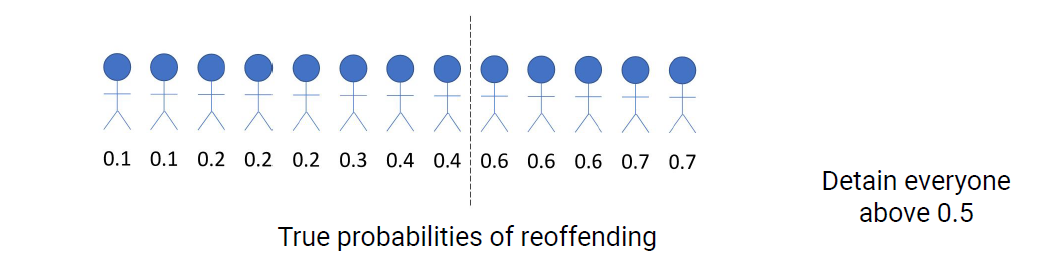
\includegraphics[width=0.8\textwidth]{figure/calibration_issue_1.png}
			\end{center}  
			%			
			\item Assume that there are two groups among the blue people:
%			
			\begin{center}
				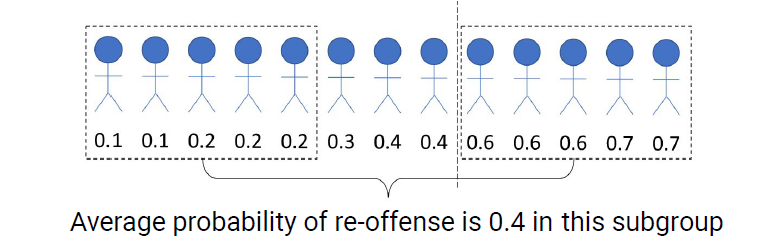
\includegraphics[width=0.5\textwidth]{figure/calibration_issue_2.png}
			\end{center}  
			%		
			
		\end{itemize}	
		\framebreak
		
		\begin{center}
			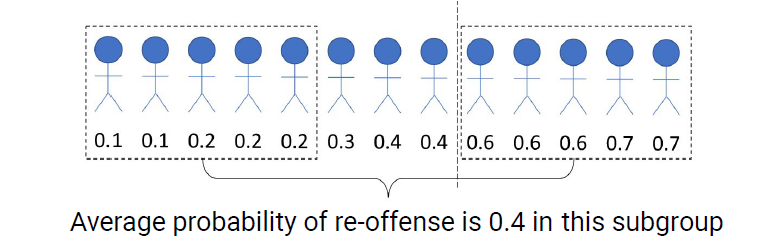
\includegraphics[width=0.5\textwidth]{figure/calibration_issue_2.png}
		\end{center}  
%		
		If we calibrate the classifier, we have no detentions any more!
%		
		\begin{center}
			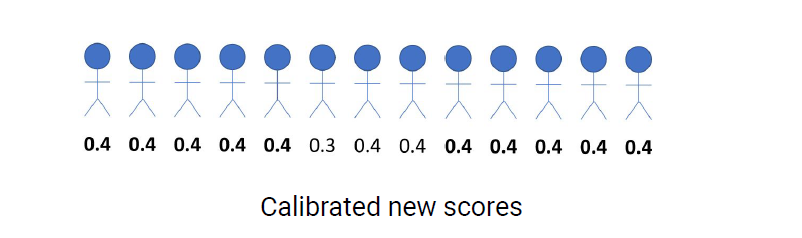
\includegraphics[width=0.7\textwidth]{figure/calibration_issue_3.png}
		\end{center}	
		%	
	}
\end{vbframe}


\begin{vbframe}{Relationships between the Fairness Criteria}
	%	
	\small{
		%	
		\begin{itemize}
			%			
			\item We have considered three fairness criteria:
			%			
			\begin{align*}
%				
				\yh &\indep \sens \tag{Independence}	\\
%				
				\yh &\indep \sens ~|~ y  \tag{Separation}\\ 
%				
				y &\indep \sens ~|~ 	\mathbf{S} \tag{Sufficiency}
%				
			\end{align*}
			%			
			%			
			\item A tempting question is how these criteria relate to each other. 
			 
			\item \textbf{(Informal) Theorem.} Any two of these criteria are mutually exclusive in general.
%			 

			\item As a consequence, we cannot impose multiple of these criteria as hard constraints on the classifier.
%			
			\item A possible solution to this issue is to consider relaxed version of these criteria as constraints.
%			
		\end{itemize}
		%	
	}
\end{vbframe}




\begin{vbframe}{Final remarks}
	%	
	\small
		%	
		\begin{itemize}
			%			
			\item Fairness is a challenging issue as also philosophers and social scientists have been trying to define it for decades.
%			
			\item Due to the increased use of ML methods in automated decision making there is a need to think about fairness in more detail.
%			
			\item  Fairness criteria such as independence, sufficiency and separation are a statistical objective way to incorporate fairness aspects into ML methods. However, on their own they are neither equivalent to a ``proof of fairness'' nor are they prefect objective functions for this purpose.
%			
			\item In summary, there are three ways to tackle the question: ``how to satisfy fairness criteria?''
%			
			\begin{enumerate}
				\small
				\item Pre-processing phase: Adjust the feature space to be uncorrelated
				with the sensitive attribute.
				\item Training phase: Build the constraint into the optimization process
				for the classifier.
				\item Post-processing phase: Adjust a learned classifier so that it is uncorrelated to the sensitive attribute.
			\end{enumerate}
			
			%			
		\end{itemize}
		%	
	
\end{vbframe}

%
\endlecture
\end{document}
